\documentclass[9pt,aspectratio=169]{beamer}

\usetheme{Madrid}
\usecolortheme{default}
\usefonttheme{professionalfonts}

\setbeamertemplate{navigation symbols}{}
\setbeamertemplate{footline}[frame number]
\setbeamercolor{block title}{bg=blue!20,fg=black}
\setbeamercolor{block body}{bg=blue!5,fg=black}

\usepackage[utf8]{inputenc}
\usepackage{amsmath}
\usepackage{booktabs}
\usepackage{array}
\usepackage{graphicx}
\usepackage{adjustbox}
\usepackage{tikz}
\usetikzlibrary{arrows.meta,positioning,shapes.geometric}

\title[MyHealthReport -- Technical Architecture]{MyHealthReport}
\subtitle{Technical Module Architecture\\ \small A modular backend design: UI, medical logic, laboratory data,\\ risk algorithms and reporting evolving independently}
\author{}
\date{24 August 2026}

\begin{document}

\begin{frame}
\titlepage
\end{frame}

\begin{frame}{Agenda}
\tiny
\tableofcontents
\end{frame}

\section{Guiding Principle}

\begin{frame}[t]{Guiding Principle}
\textcolor{black!55}{\scriptsize Modular, not screen-based}\\[2pt]
\begin{itemize}
\scriptsize
\item Do not arrange the platform purely by screen
\item Arrange into separate modules so UI, medical logic, laboratory data, risk algorithms, and reporting can each evolve independently
\item This document defines the master technical module architecture: 26 modules, grouped into 6 functional clusters
\end{itemize}
\vspace{4pt}
\begin{center}
\begin{adjustbox}{max width=0.96\linewidth,max height=0.62\textheight}
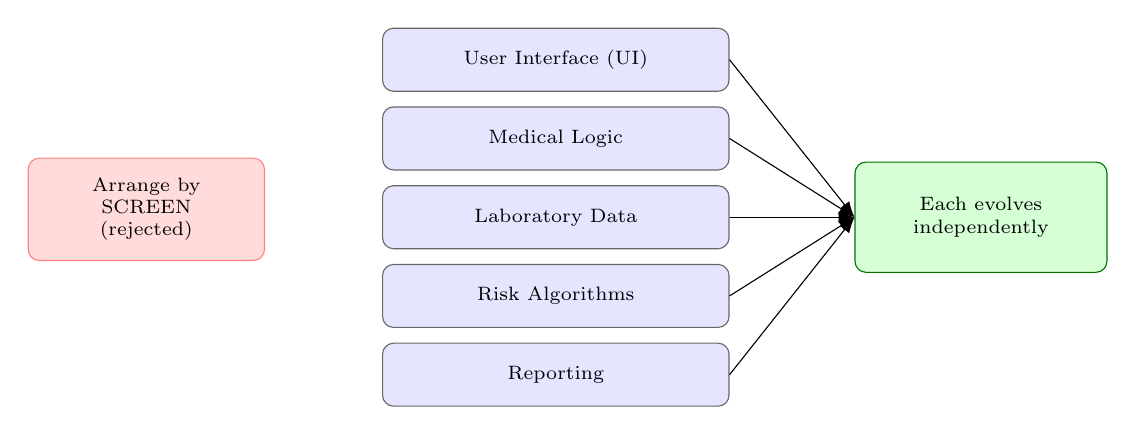
\begin{tikzpicture}[>=Latex]
\node[draw=red!50,rounded corners,fill=red!14,minimum width=3.0cm,minimum height=1.3cm,align=center,font=\scriptsize,text width=2.75cm,inner sep=2pt] (gp0) at (0,0) {Arrange by\\SCREEN\\(rejected)};
\node[draw=black!60,rounded corners,fill=blue!10,minimum width=4.4cm,minimum height=0.8cm,align=center,font=\scriptsize,text width=4.15cm,inner sep=2pt] (gp1) at (5.2,1.9) {User Interface (UI)};
\node[draw=black!60,rounded corners,fill=blue!10,minimum width=4.4cm,minimum height=0.8cm,align=center,font=\scriptsize,text width=4.15cm,inner sep=2pt] (gp2) at (5.2,0.8999999999999999) {Medical Logic};
\node[draw=black!60,rounded corners,fill=blue!10,minimum width=4.4cm,minimum height=0.8cm,align=center,font=\scriptsize,text width=4.15cm,inner sep=2pt] (gp3) at (5.2,-0.10000000000000009) {Laboratory Data};
\node[draw=black!60,rounded corners,fill=blue!10,minimum width=4.4cm,minimum height=0.8cm,align=center,font=\scriptsize,text width=4.15cm,inner sep=2pt] (gp4) at (5.2,-1.1) {Risk Algorithms};
\node[draw=black!60,rounded corners,fill=blue!10,minimum width=4.4cm,minimum height=0.8cm,align=center,font=\scriptsize,text width=4.15cm,inner sep=2pt] (gp5) at (5.2,-2.1) {Reporting};
\node[draw=green!45!black,rounded corners,fill=green!16,minimum width=3.2cm,minimum height=1.4cm,align=center,font=\scriptsize,text width=2.95cm,inner sep=2pt] (gpc) at (10.6,-0.1) {Each evolves\\independently};
\draw[-{Latex[length=2mm]}] (gp1.east)--(gpc.west);
\draw[-{Latex[length=2mm]}] (gp2.east)--(gpc.west);
\draw[-{Latex[length=2mm]}] (gp3.east)--(gpc.west);
\draw[-{Latex[length=2mm]}] (gp4.east)--(gpc.west);
\draw[-{Latex[length=2mm]}] (gp5.east)--(gpc.west);
\end{tikzpicture}
\end{adjustbox}
\end{center}
\end{frame}

\section{Master Technical Architecture}

\begin{frame}[t]{Master Technical Architecture (Modules 01--21)}
\textcolor{black!55}{\scriptsize The full pipeline, top to bottom}\\[2pt]
\begin{center}
\begin{adjustbox}{max width=0.96\linewidth,max height=0.72\textheight}
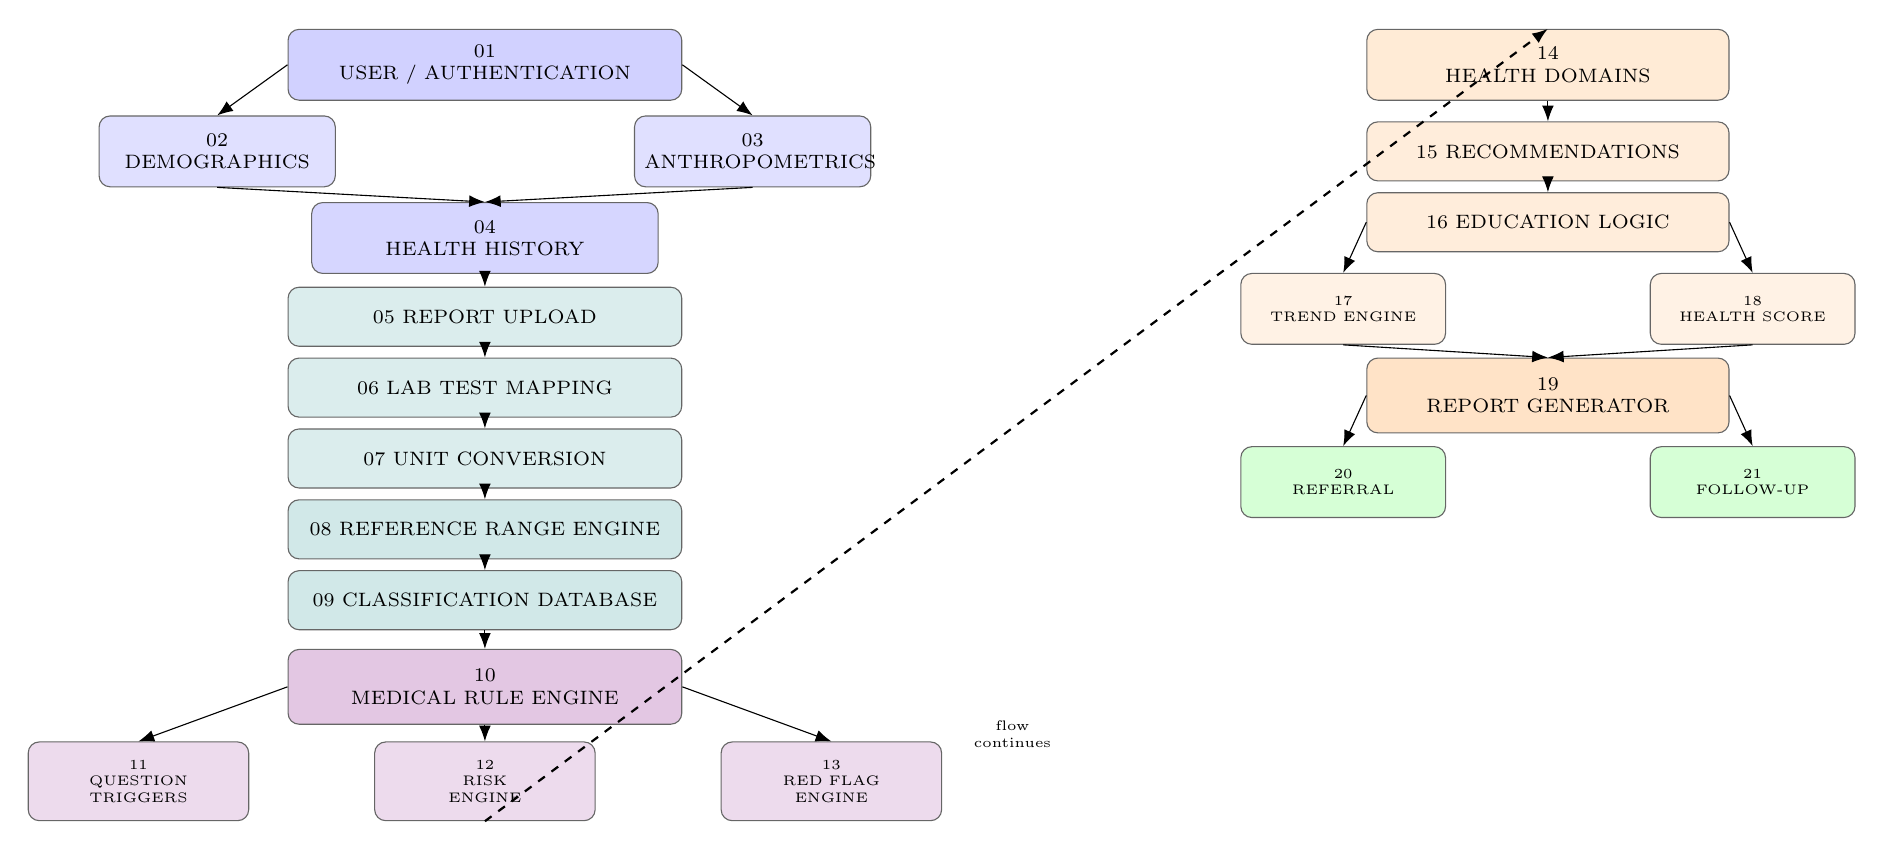
\begin{tikzpicture}[>=Latex]
\node[draw=black!60,rounded corners,fill=blue!18,minimum width=5.0cm,minimum height=0.9cm,align=center,font=\scriptsize,text width=4.75cm,inner sep=2pt] (a01) at (0,0) {01\\USER / AUTHENTICATION};
\node[draw=black!60,rounded corners,fill=blue!12,minimum width=3.0cm,minimum height=0.9cm,align=center,font=\scriptsize,text width=2.75cm,inner sep=2pt] (a02) at (-3.4,-1.1) {02\\DEMOGRAPHICS};
\node[draw=black!60,rounded corners,fill=blue!12,minimum width=3.0cm,minimum height=0.9cm,align=center,font=\scriptsize,text width=2.75cm,inner sep=2pt] (a03) at (3.4,-1.1) {03\\ANTHROPOMETRICS};
\draw[-{Latex[length=2mm]}] (a01.west)--(a02.north);
\draw[-{Latex[length=2mm]}] (a01.east)--(a03.north);
\node[draw=black!60,rounded corners,fill=blue!16,minimum width=4.4cm,minimum height=0.9cm,align=center,font=\scriptsize,text width=4.15cm,inner sep=2pt] (a04) at (0,-2.2) {04\\HEALTH HISTORY};
\draw[-{Latex[length=2mm]}] (a02.south)--(a04.north);
\draw[-{Latex[length=2mm]}] (a03.south)--(a04.north);
\node[draw=black!60,rounded corners,fill=teal!14,minimum width=5.0cm,minimum height=0.75cm,align=center,font=\scriptsize,text width=4.75cm,inner sep=2pt] (a05) at (0,-3.2) {05  REPORT UPLOAD};
\draw[-{Latex[length=2mm]}] (a04.south)--(a05.north);
\node[draw=black!60,rounded corners,fill=teal!14,minimum width=5.0cm,minimum height=0.75cm,align=center,font=\scriptsize,text width=4.75cm,inner sep=2pt] (a06) at (0,-4.1) {06  LAB TEST MAPPING};
\draw[-{Latex[length=2mm]}] (a05.south)--(a06.north);
\node[draw=black!60,rounded corners,fill=teal!14,minimum width=5.0cm,minimum height=0.75cm,align=center,font=\scriptsize,text width=4.75cm,inner sep=2pt] (a07) at (0,-5.0) {07  UNIT CONVERSION};
\draw[-{Latex[length=2mm]}] (a06.south)--(a07.north);
\node[draw=black!60,rounded corners,fill=teal!18,minimum width=5.0cm,minimum height=0.75cm,align=center,font=\scriptsize,text width=4.75cm,inner sep=2pt] (a08) at (0,-5.9) {08  REFERENCE RANGE ENGINE};
\draw[-{Latex[length=2mm]}] (a07.south)--(a08.north);
\node[draw=black!60,rounded corners,fill=teal!18,minimum width=5.0cm,minimum height=0.75cm,align=center,font=\scriptsize,text width=4.75cm,inner sep=2pt] (a09) at (0,-6.8) {09  CLASSIFICATION DATABASE};
\draw[-{Latex[length=2mm]}] (a08.south)--(a09.north);
\node[draw=black!60,rounded corners,fill=violet!22,minimum width=5.0cm,minimum height=0.95cm,align=center,font=\scriptsize,text width=4.75cm,inner sep=2pt] (a10) at (0,-7.9) {10\\MEDICAL RULE ENGINE};
\draw[-{Latex[length=2mm]}] (a09.south)--(a10.north);
\node[draw=black!60,rounded corners,fill=violet!14,minimum width=2.8cm,minimum height=1.0cm,align=center,font=\tiny,text width=2.55cm,inner sep=2pt] (a11) at (-4.4,-9.1) {11\\QUESTION\\TRIGGERS};
\node[draw=black!60,rounded corners,fill=violet!14,minimum width=2.8cm,minimum height=1.0cm,align=center,font=\tiny,text width=2.55cm,inner sep=2pt] (a12) at (0,-9.1) {12\\RISK\\ENGINE};
\node[draw=black!60,rounded corners,fill=violet!14,minimum width=2.8cm,minimum height=1.0cm,align=center,font=\tiny,text width=2.55cm,inner sep=2pt] (a13) at (4.4,-9.1) {13\\RED FLAG\\ENGINE};
\draw[-{Latex[length=2mm]}] (a10.west)--(a11.north);
\draw[-{Latex[length=2mm]}] (a10.south)--(a12.north);
\draw[-{Latex[length=2mm]}] (a10.east)--(a13.north);
\node[draw=black!60,rounded corners,fill=orange!16,minimum width=4.6cm,minimum height=0.9cm,align=center,font=\scriptsize,text width=4.35cm,inner sep=2pt] (a14) at (13.5,0) {14\\HEALTH DOMAINS};
\node[draw=black!60,rounded corners,fill=orange!14,minimum width=4.6cm,minimum height=0.75cm,align=center,font=\scriptsize,text width=4.35cm,inner sep=2pt] (a15) at (13.5,-1.1) {15  RECOMMENDATIONS};
\draw[-{Latex[length=2mm]}] (a14.south)--(a15.north);
\node[draw=black!60,rounded corners,fill=orange!14,minimum width=4.6cm,minimum height=0.75cm,align=center,font=\scriptsize,text width=4.35cm,inner sep=2pt] (a16) at (13.5,-2.0) {16  EDUCATION LOGIC};
\draw[-{Latex[length=2mm]}] (a15.south)--(a16.north);
\node[draw=black!60,rounded corners,fill=orange!10,minimum width=2.6cm,minimum height=0.9cm,align=center,font=\tiny,text width=2.35cm,inner sep=2pt] (a17) at (10.9,-3.1) {17\\TREND ENGINE};
\node[draw=black!60,rounded corners,fill=orange!10,minimum width=2.6cm,minimum height=0.9cm,align=center,font=\tiny,text width=2.35cm,inner sep=2pt] (a18) at (16.1,-3.1) {18\\HEALTH SCORE};
\draw[-{Latex[length=2mm]}] (a16.west)--(a17.north);
\draw[-{Latex[length=2mm]}] (a16.east)--(a18.north);
\node[draw=black!60,rounded corners,fill=orange!22,minimum width=4.6cm,minimum height=0.95cm,align=center,font=\scriptsize,text width=4.35cm,inner sep=2pt] (a19) at (13.5,-4.2) {19\\REPORT GENERATOR};
\draw[-{Latex[length=2mm]}] (a17.south)--(a19.north);
\draw[-{Latex[length=2mm]}] (a18.south)--(a19.north);
\node[draw=black!60,rounded corners,fill=green!16,minimum width=2.6cm,minimum height=0.9cm,align=center,font=\tiny,text width=2.35cm,inner sep=2pt] (a20) at (10.9,-5.3) {20\\REFERRAL};
\node[draw=black!60,rounded corners,fill=green!16,minimum width=2.6cm,minimum height=0.9cm,align=center,font=\tiny,text width=2.35cm,inner sep=2pt] (a21) at (16.1,-5.3) {21\\FOLLOW-UP};
\draw[-{Latex[length=2mm]}] (a19.west)--(a20.north);
\draw[-{Latex[length=2mm]}] (a19.east)--(a21.north);
\draw[-{Latex[length=2mm]},dashed,thick] (a12.south)--(a14.north);
\node[font=\tiny,align=center] at (6.7,-8.5) {flow\\continues};
\end{tikzpicture}
\end{adjustbox}
\end{center}
\end{frame}

\begin{frame}[t]{System-Wide Governance Layer (Modules 22--26)}
\textcolor{black!55}{\scriptsize Five modules underlying the entire pipeline}\\[2pt]
\begin{center}
\begin{adjustbox}{max width=0.96\linewidth,max height=0.6\textheight}
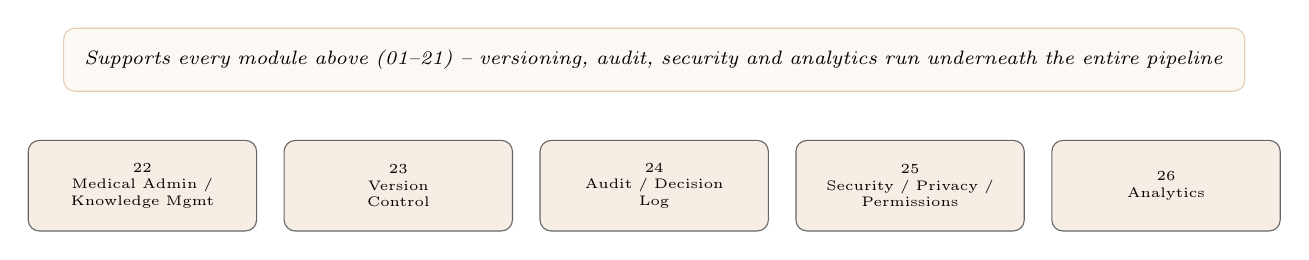
\begin{tikzpicture}[>=Latex]
\node[draw=black!60,rounded corners,fill=brown!14,minimum width=2.9cm,minimum height=1.15cm,align=center,font=\tiny,text width=2.65cm,inner sep=2pt] (g0) at (0.0,0.0) {22\\Medical Admin /\\Knowledge Mgmt};
\node[draw=black!60,rounded corners,fill=brown!14,minimum width=2.9cm,minimum height=1.15cm,align=center,font=\tiny,text width=2.65cm,inner sep=2pt] (g1) at (3.25,0.0) {23\\Version\\Control};
\node[draw=black!60,rounded corners,fill=brown!14,minimum width=2.9cm,minimum height=1.15cm,align=center,font=\tiny,text width=2.65cm,inner sep=2pt] (g2) at (6.5,0.0) {24\\Audit / Decision\\Log};
\node[draw=black!60,rounded corners,fill=brown!14,minimum width=2.9cm,minimum height=1.15cm,align=center,font=\tiny,text width=2.65cm,inner sep=2pt] (g3) at (9.75,0.0) {25\\Security / Privacy /\\Permissions};
\node[draw=black!60,rounded corners,fill=brown!14,minimum width=2.9cm,minimum height=1.15cm,align=center,font=\tiny,text width=2.65cm,inner sep=2pt] (g4) at (13.0,0.0) {26\\Analytics};
\node[draw=brown!40,rounded corners,fill=brown!5,minimum width=15.0cm,minimum height=0.8cm,align=center,font=\scriptsize,text width=14.75cm,inner sep=2pt] (gov_note) at (6.5,1.6) {\textit{Supports every module above (01--21) -- versioning, audit, security and analytics run underneath the entire pipeline}};
\end{tikzpicture}
\end{adjustbox}
\end{center}
\end{frame}

\section{Cluster 1 -- Identity \& Profile (M1--M4)}

\begin{frame}[t]{Module 1: User Access \& Welcome Module}
\textcolor{black!55}{\scriptsize Cluster 1 -- \textcolor{blue}{\textbf{Identity \& Profile}} (M1--M4) \\ Every intake screen resolves into one identity}\\[2pt]
\begin{itemize}
\scriptsize
\item Entry layer: landing, registration, login, verification, consent, privacy, terms, disclaimer, account settings, language
\item Main output: \texttt{USER\_ID}
\item Almost everything afterward links back to this one ID
\end{itemize}
\vspace{4pt}
\begin{center}
\begin{adjustbox}{max width=0.96\linewidth,max height=0.62\textheight}
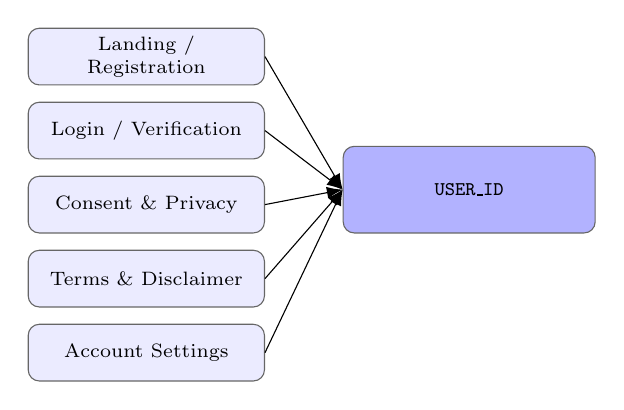
\begin{tikzpicture}[>=Latex]
\node[draw=black!60,rounded corners,fill=blue!8,minimum width=3.0cm,minimum height=0.72cm,align=center,font=\scriptsize,text width=2.75cm,inner sep=2pt] (hi0) at (0,0) {Landing / Registration};
\node[draw=black!60,rounded corners,fill=blue!8,minimum width=3.0cm,minimum height=0.72cm,align=center,font=\scriptsize,text width=2.75cm,inner sep=2pt] (hi1) at (0,-0.94) {Login / Verification};
\node[draw=black!60,rounded corners,fill=blue!8,minimum width=3.0cm,minimum height=0.72cm,align=center,font=\scriptsize,text width=2.75cm,inner sep=2pt] (hi2) at (0,-1.88) {Consent \& Privacy};
\node[draw=black!60,rounded corners,fill=blue!8,minimum width=3.0cm,minimum height=0.72cm,align=center,font=\scriptsize,text width=2.75cm,inner sep=2pt] (hi3) at (0,-2.82) {Terms \& Disclaimer};
\node[draw=black!60,rounded corners,fill=blue!8,minimum width=3.0cm,minimum height=0.72cm,align=center,font=\scriptsize,text width=2.75cm,inner sep=2pt] (hi4) at (0,-3.76) {Account Settings};
\node[draw=black!60,rounded corners,fill=blue!30,minimum width=3.2cm,minimum height=1.1cm,align=center,font=\scriptsize,text width=2.95cm,inner sep=2pt] (hic) at (4.1,-1.6899999999999997) {\texttt{USER\_ID}};
\draw[-{Latex[length=2mm]}] (hi0.east)--(hic.west);
\draw[-{Latex[length=2mm]}] (hi1.east)--(hic.west);
\draw[-{Latex[length=2mm]}] (hi2.east)--(hic.west);
\draw[-{Latex[length=2mm]}] (hi3.east)--(hic.west);
\draw[-{Latex[length=2mm]}] (hi4.east)--(hic.west);
\end{tikzpicture}
\end{adjustbox}
\end{center}
\end{frame}

\begin{frame}[t]{Module 2: Basic Demographic Profile Module}
\textcolor{black!55}{\scriptsize Cluster 1 -- \textcolor{blue}{\textbf{Identity \& Profile}} (M1--M4) \\ One demographic value, reused by four downstream engines}\\[2pt]
\begin{itemize}
\scriptsize
\item Stores DOB, calculated age, biological sex, ethnicity (where relevant), region, pregnancy/menopausal status
\item Becomes part of the shared risk-variable database
\end{itemize}
\vspace{4pt}
\begin{center}
\begin{adjustbox}{max width=0.96\linewidth,max height=0.62\textheight}
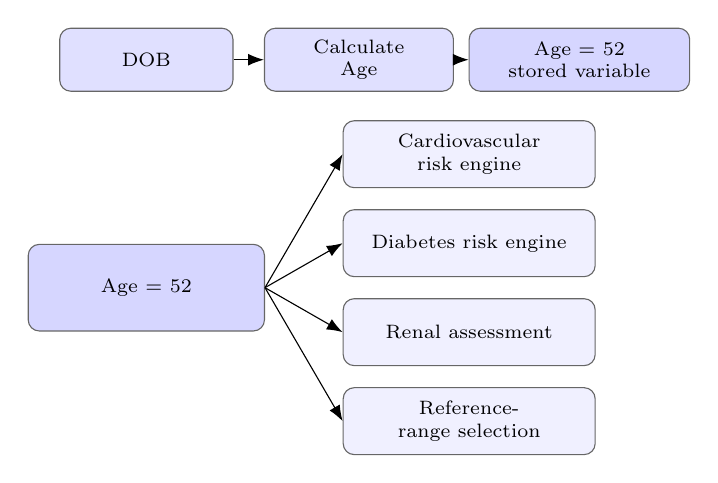
\begin{tikzpicture}[>=Latex]
\node[draw=black!60,rounded corners,fill=blue!12,minimum width=2.2cm,minimum height=0.8cm,align=center,font=\scriptsize,text width=1.9500000000000002cm,inner sep=2pt] (d1) at (0,0) {DOB};
\node[draw=black!60,rounded corners,fill=blue!12,minimum width=2.4cm,minimum height=0.8cm,align=center,font=\scriptsize,text width=2.15cm,inner sep=2pt] (d2) at (2.7,0) {Calculate\\Age};
\node[draw=black!60,rounded corners,fill=blue!16,minimum width=2.8cm,minimum height=0.8cm,align=center,font=\scriptsize,text width=2.55cm,inner sep=2pt] (d3) at (5.5,0) {Age = 52\\stored variable};
\draw[-{Latex[length=2mm]}] (d1.east)--(d2.west);
\draw[-{Latex[length=2mm]}] (d2.east)--(d3.west);
\begin{scope}[shift={(0,-1.2)}]
\node[draw=black!60,rounded corners,fill=blue!16,minimum width=3.0cm,minimum height=1.1cm,align=center,font=\scriptsize,text width=2.75cm,inner sep=2pt] (d4c) at (0,-1.695) {Age = 52};
\node[draw=black!60,rounded corners,fill=blue!6,minimum width=3.2cm,minimum height=0.85cm,align=center,font=\scriptsize,text width=2.95cm,inner sep=2pt] (d40) at (4.1,0) {Cardiovascular risk engine};
\draw[-{Latex[length=2mm]}] (d4c.east)--(d40.west);
\node[draw=black!60,rounded corners,fill=blue!6,minimum width=3.2cm,minimum height=0.85cm,align=center,font=\scriptsize,text width=2.95cm,inner sep=2pt] (d41) at (4.1,-1.13) {Diabetes risk engine};
\draw[-{Latex[length=2mm]}] (d4c.east)--(d41.west);
\node[draw=black!60,rounded corners,fill=blue!6,minimum width=3.2cm,minimum height=0.85cm,align=center,font=\scriptsize,text width=2.95cm,inner sep=2pt] (d42) at (4.1,-2.26) {Renal assessment};
\draw[-{Latex[length=2mm]}] (d4c.east)--(d42.west);
\node[draw=black!60,rounded corners,fill=blue!6,minimum width=3.2cm,minimum height=0.85cm,align=center,font=\scriptsize,text width=2.95cm,inner sep=2pt] (d43) at (4.1,-3.3899999999999997) {Reference-range selection};
\draw[-{Latex[length=2mm]}] (d4c.east)--(d43.west);
\end{scope}
\end{tikzpicture}
\end{adjustbox}
\end{center}
\end{frame}

\begin{frame}[t]{Module 3: Anthropometric Profile Module}
\textcolor{black!55}{\scriptsize Cluster 1 -- \textcolor{blue}{\textbf{Identity \& Profile}} (M1--M4) \\ Four layers, stored separately, so guideline updates never touch raw data}\\[2pt]
\begin{itemize}
\scriptsize
\item Own module because it produces longitudinal anthropometric trends
\item Raw: height, weight, waist/hip circumference, BP, heart rate, body composition
\item Derived: BMI, BMI category, waist-height/waist-hip ratio, central obesity, BP classification, weight change \%
\item \textbf{Key rule: raw data and calculated classifications are stored separately}
\end{itemize}
\vspace{4pt}
\begin{center}
\begin{adjustbox}{max width=0.96\linewidth,max height=0.62\textheight}
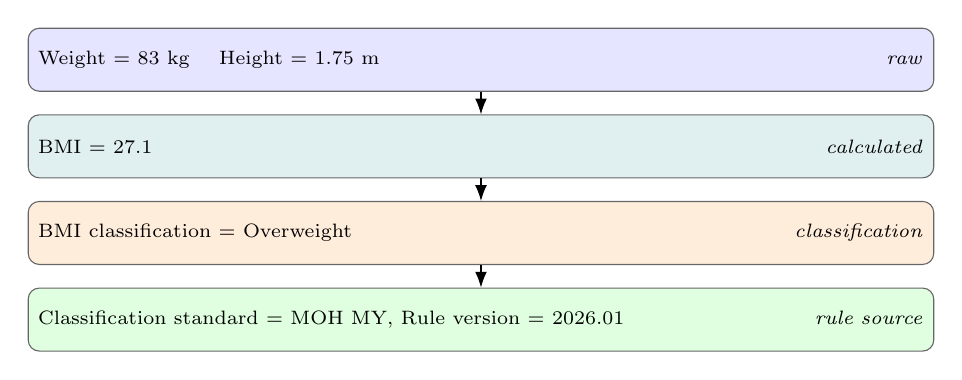
\begin{tikzpicture}[>=Latex]
\node[draw=black!60,rounded corners,fill=blue!10,minimum width=11.5cm,minimum height=0.8cm,align=center,font=\scriptsize,text width=11.25cm,inner sep=2pt] (lv0) at (0,0) {Weight = 83~kg \quad Height = 1.75~m \hfill \textit{raw}};
\node[draw=black!60,rounded corners,fill=teal!12,minimum width=11.5cm,minimum height=0.8cm,align=center,font=\scriptsize,text width=11.25cm,inner sep=2pt] (lv1) at (0,-1.1) {BMI = 27.1 \hfill \textit{calculated}};
\node[draw=black!60,rounded corners,fill=orange!14,minimum width=11.5cm,minimum height=0.8cm,align=center,font=\scriptsize,text width=11.25cm,inner sep=2pt] (lv2) at (0,-2.2) {BMI classification = Overweight \hfill \textit{classification}};
\node[draw=black!60,rounded corners,fill=green!12,minimum width=11.5cm,minimum height=0.8cm,align=center,font=\scriptsize,text width=11.25cm,inner sep=2pt] (lv3) at (0,-3.3000000000000003) {Classification standard = MOH MY, Rule version = 2026.01 \hfill \textit{rule source}};
\draw[-{Latex[length=2mm]}] (lv0.south)--(lv1.north);
\draw[-{Latex[length=2mm]}] (lv1.south)--(lv2.north);
\draw[-{Latex[length=2mm]}] (lv2.south)--(lv3.north);
\end{tikzpicture}
\end{adjustbox}
\end{center}
\end{frame}

\begin{frame}[t]{Module 4: Health History Module}
\textcolor{black!55}{\scriptsize Cluster 1 -- \textcolor{blue}{\textbf{Identity \& Profile}} (M1--M4) \\ Progressive categories, each answerable in four defined states}\\[2pt]
\begin{itemize}
\scriptsize
\item Progressive collection, not all at registration: medical/family history, medication, supplements, allergy, smoking, alcohol, exercise, diet, sleep, stress, prior CVD/diabetes/hypertension/kidney/liver disease
\item \textbf{Answer states: UNKNOWN / YES / NO / NOT APPLICABLE} -- never let NULL mean everything
\end{itemize}
\vspace{4pt}
\begin{center}
\begin{adjustbox}{max width=0.96\linewidth,max height=0.62\textheight}
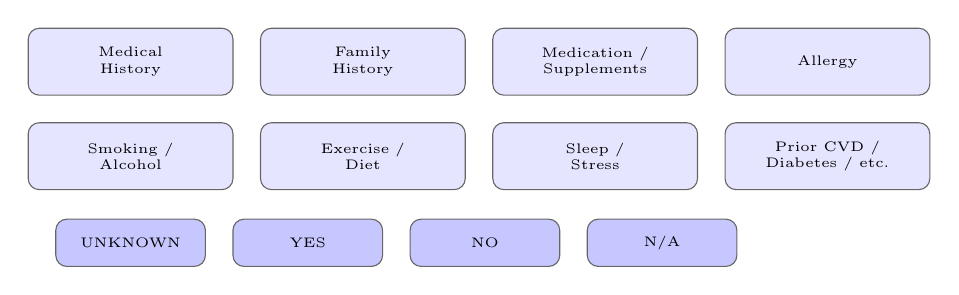
\begin{tikzpicture}[>=Latex]
\node[draw=black!60,rounded corners,fill=blue!10,minimum width=2.6cm,minimum height=0.85cm,align=center,font=\tiny,text width=2.35cm,inner sep=2pt] (g0) at (0.0,0.0) {Medical\\History};
\node[draw=black!60,rounded corners,fill=blue!10,minimum width=2.6cm,minimum height=0.85cm,align=center,font=\tiny,text width=2.35cm,inner sep=2pt] (g1) at (2.95,0.0) {Family\\History};
\node[draw=black!60,rounded corners,fill=blue!10,minimum width=2.6cm,minimum height=0.85cm,align=center,font=\tiny,text width=2.35cm,inner sep=2pt] (g2) at (5.9,0.0) {Medication /\\Supplements};
\node[draw=black!60,rounded corners,fill=blue!10,minimum width=2.6cm,minimum height=0.85cm,align=center,font=\tiny,text width=2.35cm,inner sep=2pt] (g3) at (8.850000000000001,0.0) {Allergy};
\node[draw=black!60,rounded corners,fill=blue!10,minimum width=2.6cm,minimum height=0.85cm,align=center,font=\tiny,text width=2.35cm,inner sep=2pt] (g4) at (0.0,-1.2) {Smoking /\\Alcohol};
\node[draw=black!60,rounded corners,fill=blue!10,minimum width=2.6cm,minimum height=0.85cm,align=center,font=\tiny,text width=2.35cm,inner sep=2pt] (g5) at (2.95,-1.2) {Exercise /\\Diet};
\node[draw=black!60,rounded corners,fill=blue!10,minimum width=2.6cm,minimum height=0.85cm,align=center,font=\tiny,text width=2.35cm,inner sep=2pt] (g6) at (5.9,-1.2) {Sleep /\\Stress};
\node[draw=black!60,rounded corners,fill=blue!10,minimum width=2.6cm,minimum height=0.85cm,align=center,font=\tiny,text width=2.35cm,inner sep=2pt] (g7) at (8.850000000000001,-1.2) {Prior CVD /\\Diabetes / etc.};
\begin{scope}[shift={(0,-2.3)}]
\node[draw=black!60,rounded corners,fill=blue!22,minimum width=1.9cm,minimum height=0.6cm,align=center,font=\tiny,text width=1.65cm,inner sep=2pt] (ans0) at (0.0,0.0) {UNKNOWN};
\node[draw=black!60,rounded corners,fill=blue!22,minimum width=1.9cm,minimum height=0.6cm,align=center,font=\tiny,text width=1.65cm,inner sep=2pt] (ans1) at (2.25,0.0) {YES};
\node[draw=black!60,rounded corners,fill=blue!22,minimum width=1.9cm,minimum height=0.6cm,align=center,font=\tiny,text width=1.65cm,inner sep=2pt] (ans2) at (4.5,0.0) {NO};
\node[draw=black!60,rounded corners,fill=blue!22,minimum width=1.9cm,minimum height=0.6cm,align=center,font=\tiny,text width=1.65cm,inner sep=2pt] (ans3) at (6.75,0.0) {N/A};
\end{scope}
\end{tikzpicture}
\end{adjustbox}
\end{center}
\end{frame}

\section{Cluster 2 -- Data Ingestion \& Standardisation (M5--M9)}

\begin{frame}[t]{Module 5: Blood Report Upload Module}
\textcolor{black!55}{\scriptsize Cluster 2 -- \textcolor{teal}{\textbf{Data Ingestion \& Standardisation}} (M5--M9) \\ Nine-step ingestion pipeline}\\[2pt]
\begin{itemize}
\scriptsize
\item The ingestion layer: upload $\to$ identify lab/date/metadata $\to$ extract analytes $\to$ map to standardized codes $\to$ capture test/result/unit/range/flag $\to$ verify $\to$ store
\item Design the database as though every result eventually becomes structured data, even before OCR is fully automated
\end{itemize}
\vspace{4pt}
\begin{center}
\begin{adjustbox}{max width=0.96\linewidth,max height=0.62\textheight}
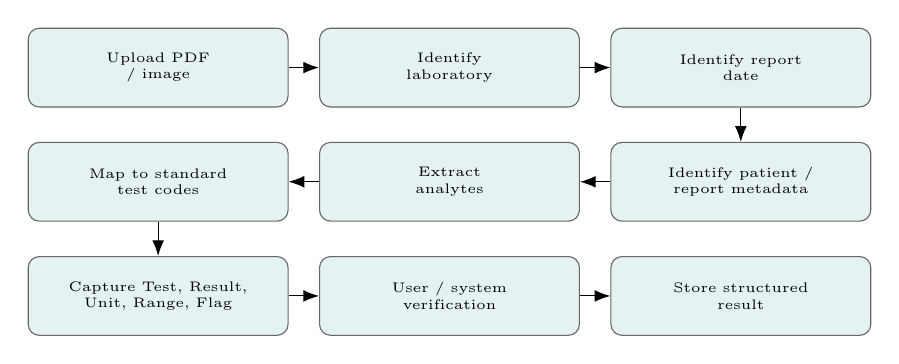
\begin{tikzpicture}[>=Latex]
\node[draw=black!60,rounded corners,fill=teal!10,minimum width=3.3cm,minimum height=1.0cm,align=center,font=\tiny,text width=3.05cm,inner sep=2pt] (s0) at (0.0,0.0) {Upload PDF\\/ image};
\node[draw=black!60,rounded corners,fill=teal!10,minimum width=3.3cm,minimum height=1.0cm,align=center,font=\tiny,text width=3.05cm,inner sep=2pt] (s1) at (3.6999999999999997,0.0) {Identify\\laboratory};
\node[draw=black!60,rounded corners,fill=teal!10,minimum width=3.3cm,minimum height=1.0cm,align=center,font=\tiny,text width=3.05cm,inner sep=2pt] (s2) at (7.3999999999999995,0.0) {Identify report\\date};
\node[draw=black!60,rounded corners,fill=teal!10,minimum width=3.3cm,minimum height=1.0cm,align=center,font=\tiny,text width=3.05cm,inner sep=2pt] (s3) at (7.3999999999999995,-1.45) {Identify patient /\\report metadata};
\node[draw=black!60,rounded corners,fill=teal!10,minimum width=3.3cm,minimum height=1.0cm,align=center,font=\tiny,text width=3.05cm,inner sep=2pt] (s4) at (3.6999999999999997,-1.45) {Extract\\analytes};
\node[draw=black!60,rounded corners,fill=teal!10,minimum width=3.3cm,minimum height=1.0cm,align=center,font=\tiny,text width=3.05cm,inner sep=2pt] (s5) at (0.0,-1.45) {Map to standard\\test codes};
\node[draw=black!60,rounded corners,fill=teal!10,minimum width=3.3cm,minimum height=1.0cm,align=center,font=\tiny,text width=3.05cm,inner sep=2pt] (s6) at (0.0,-2.9) {Capture Test, Result,\\Unit, Range, Flag};
\node[draw=black!60,rounded corners,fill=teal!10,minimum width=3.3cm,minimum height=1.0cm,align=center,font=\tiny,text width=3.05cm,inner sep=2pt] (s7) at (3.6999999999999997,-2.9) {User / system\\verification};
\node[draw=black!60,rounded corners,fill=teal!10,minimum width=3.3cm,minimum height=1.0cm,align=center,font=\tiny,text width=3.05cm,inner sep=2pt] (s8) at (7.3999999999999995,-2.9) {Store structured\\result};
\draw[-{Latex[length=2mm]}] (s0.east)--(s1.west);
\draw[-{Latex[length=2mm]}] (s1.east)--(s2.west);
\draw[-{Latex[length=2mm]}] (s2.south)--(s3.north);
\draw[-{Latex[length=2mm]}] (s3.west)--(s4.east);
\draw[-{Latex[length=2mm]}] (s4.west)--(s5.east);
\draw[-{Latex[length=2mm]}] (s5.south)--(s6.north);
\draw[-{Latex[length=2mm]}] (s6.east)--(s7.west);
\draw[-{Latex[length=2mm]}] (s7.east)--(s8.west);
\end{tikzpicture}
\end{adjustbox}
\end{center}
\end{frame}

\begin{frame}[t]{Module 5: Blood Report Upload Module}
\textcolor{black!55}{\scriptsize One fully structured result}\\[2pt]
\begin{center}\scriptsize
\begin{tabular}{ll}
\toprule
\textbf{Field} & \textbf{Value} \\
\midrule
Test & ALT \\
Value & 68 \\
Unit & U/L \\
Lab lower limit & 0 \\
Lab upper limit & 41 \\
Lab & XYZ Laboratory \\
Date & 2026-08-20 \\
\bottomrule
\end{tabular}
\end{center}
\end{frame}

\begin{frame}[t]{Module 6: Laboratory Test Master Database}
\textcolor{black!55}{\scriptsize Cluster 2 -- \textcolor{teal}{\textbf{Data Ingestion \& Standardisation}} (M5--M9) \\ Standardized dictionary example}\\[2pt]
\begin{itemize}
\scriptsize
\item Standardized Lab Test Dictionary solves inconsistent lab naming conventions
\item Downstream algorithms reference the internal code (e.g. \texttt{LAB\_HBA1C}) -- never the raw report text
\end{itemize}
\vspace{4pt}
\begin{center}\scriptsize
\begin{tabular}{lll}
\toprule
\textbf{Internal Code} & \textbf{Standard Name} & \textbf{Alternate Names} \\
\midrule
\texttt{LAB\_GLU\_FAST} & Fasting Plasma Glucose & FBS, FPG \\
\texttt{LAB\_HBA1C} & HbA1c & Glycated Hb \\
\texttt{LAB\_ALT} & ALT & SGPT \\
\texttt{LAB\_AST} & AST & SGOT \\
\texttt{LAB\_CREAT} & Creatinine & Serum Creatinine \\
\bottomrule
\end{tabular}
\end{center}
\end{frame}

\begin{frame}[t]{Module 7: Unit Standardisation \& Conversion Module}
\textcolor{black!55}{\scriptsize Cluster 2 -- \textcolor{teal}{\textbf{Data Ingestion \& Standardisation}} (M5--M9) \\ Glucose example -- both values are kept}\\[2pt]
\begin{itemize}
\scriptsize
\item Algorithms must never consume whatever unit the lab happens to report
\item Original result + original unit is preserved; a canonical value + canonical unit is derived alongside it
\item \textbf{Never overwrite the original laboratory value}
\end{itemize}
\vspace{4pt}
\begin{center}
\begin{adjustbox}{max width=0.96\linewidth,max height=0.62\textheight}
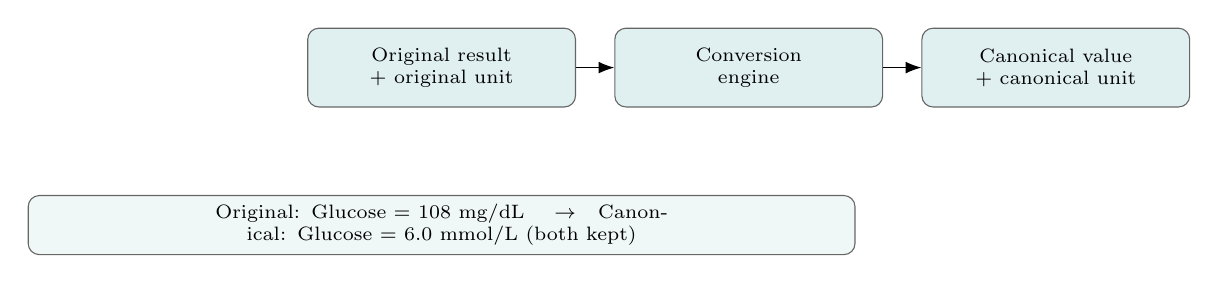
\begin{tikzpicture}[>=Latex]
\node[draw=black!60,rounded corners,fill=teal!12,minimum width=3.4cm,minimum height=1.0cm,align=center,font=\scriptsize,text width=3.15cm,inner sep=2pt] (h0) at (0,0) {Original result\\+ original unit};
\node[draw=black!60,rounded corners,fill=teal!12,minimum width=3.4cm,minimum height=1.0cm,align=center,font=\scriptsize,text width=3.15cm,inner sep=2pt] (h1) at (3.9,0) {Conversion\\engine};
\node[draw=black!60,rounded corners,fill=teal!12,minimum width=3.4cm,minimum height=1.0cm,align=center,font=\scriptsize,text width=3.15cm,inner sep=2pt] (h2) at (7.8,0) {Canonical value\\+ canonical unit};
\draw[-{Latex[length=2mm]}] (h0.east)--(h1.west);
\draw[-{Latex[length=2mm]}] (h1.east)--(h2.west);
\node[draw=black!60,rounded corners,fill=teal!6,minimum width=10.5cm,minimum height=0.75cm,align=center,font=\scriptsize,text width=10.25cm,inner sep=2pt] (u_ex) at (0,-2.0) {Original: Glucose = 108 mg/dL \quad$\to$\quad Canonical: Glucose = 6.0 mmol/L (both kept)};
\end{tikzpicture}
\end{adjustbox}
\end{center}
\end{frame}

\begin{frame}[t]{Module 8: Laboratory Reference Range Database}
\textcolor{black!55}{\scriptsize Cluster 2 -- \textcolor{teal}{\textbf{Data Ingestion \& Standardisation}} (M5--M9) \\ Two distinct questions, two distinct databases}\\[2pt]
\begin{itemize}
\scriptsize
\item Separate from the disease/risk classification database
\item Stores lab, test, limits, unit, sex/age/pregnancy criteria, method, effective date, version
\item Answers ``is this outside the \emph{lab's} range?'' -- a different question from ``does this meet a \emph{clinical} threshold?''
\end{itemize}
\vspace{4pt}
\begin{center}
\begin{adjustbox}{max width=0.96\linewidth,max height=0.62\textheight}
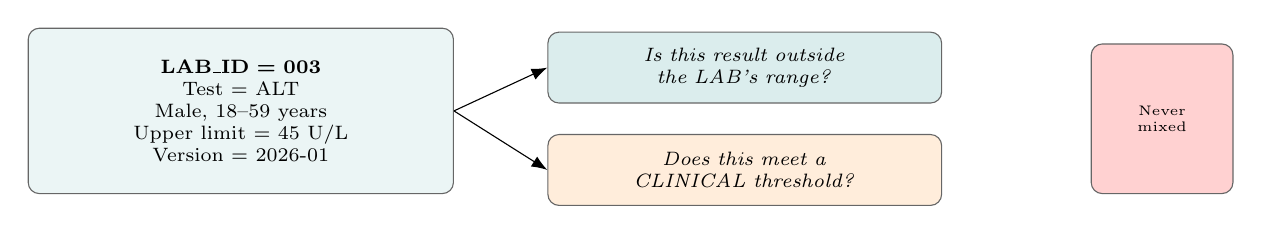
\begin{tikzpicture}[>=Latex]
\node[draw=black!60,rounded corners,fill=teal!8,minimum width=5.4cm,minimum height=2.1cm,align=center,font=\scriptsize,text width=5.15cm,inner sep=2pt] (rr1) at (0,0) {\textbf{LAB\_ID = 003}\\Test = ALT\\Male, 18--59 years\\Upper limit = 45 U/L\\Version = 2026-01};
\node[draw=black!60,rounded corners,fill=teal!14,minimum width=5.0cm,minimum height=0.9cm,align=center,font=\scriptsize,text width=4.75cm,inner sep=2pt] (rr2) at (6.4,0.55) {\textit{Is this result outside}\\\textit{the LAB's range?}};
\node[draw=black!60,rounded corners,fill=orange!14,minimum width=5.0cm,minimum height=0.9cm,align=center,font=\scriptsize,text width=4.75cm,inner sep=2pt] (rr3) at (6.4,-0.75) {\textit{Does this meet a}\\\textit{CLINICAL threshold?}};
\node[draw=black!60,rounded corners,fill=red!18,minimum width=1.8cm,minimum height=1.9cm,align=center,font=\tiny,text width=1.55cm,inner sep=2pt] (rr4) at (11.7,-0.1) {Never\\mixed};
\draw[-{Latex[length=2mm]}] (rr1.east)--(rr2.west);
\draw[-{Latex[length=2mm]}] (rr1.east)--(rr3.west);
\end{tikzpicture}
\end{adjustbox}
\end{center}
\end{frame}

\begin{frame}[t]{Module 9: Clinical Classification Standard Database}
\textcolor{black!55}{\scriptsize Cluster 2 -- \textcolor{teal}{\textbf{Data Ingestion \& Standardisation}} (M5--M9) \\ One classification rule, fully specified as metadata}\\[2pt]
\begin{itemize}
\scriptsize
\item Where medical guidelines are stored: BMI, BP, HbA1c, fasting glucose, LDL, triglyceride, eGFR, albuminuria, anaemia, liver enzyme classifications, etc.
\item Every rule carries full metadata -- this becomes the medical knowledge database
\end{itemize}
\vspace{4pt}
\begin{center}
\begin{adjustbox}{max width=0.96\linewidth,max height=0.62\textheight}
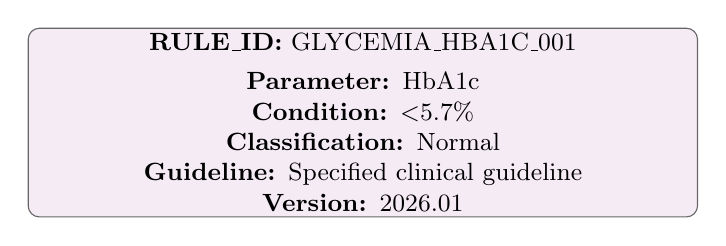
\begin{tikzpicture}[>=Latex]
\node[draw=black!60,rounded corners,fill=violet!8,minimum width=8.5cm,minimum height=2.3cm,align=center,font=\small,text width=8.25cm,inner sep=2pt] (rule_card) at (0,0) {\textbf{RULE\_ID:} GLYCEMIA\_HBA1C\_001\\[3pt]\textbf{Parameter:} HbA1c\\\textbf{Condition:} $<$5.7\%\\\textbf{Classification:} Normal\\\textbf{Guideline:} Specified clinical guideline\\\textbf{Version:} 2026.01};
\end{tikzpicture}
\end{adjustbox}
\end{center}
\end{frame}

\section{Cluster 3 -- Medical Intelligence Core (M10--M13)}

\begin{frame}[t]{Module 10: Rule Engine / Medical Logic Engine}
\textcolor{black!55}{\scriptsize Cluster 3 -- \textcolor{violet}{\textbf{Medical Intelligence Core}} (M10--M13) \\ Five inputs, five outputs, one engine}\\[2pt]
\begin{itemize}
\scriptsize
\item \textbf{The heart of the platform} -- medical decisions must never be coded directly into individual screens
\item Combines patient, anthropometric, lab, history and medication data into classifications, risk flags, question triggers, recommendations and referral triggers
\end{itemize}
\vspace{4pt}
\begin{center}
\begin{adjustbox}{max width=0.96\linewidth,max height=0.62\textheight}
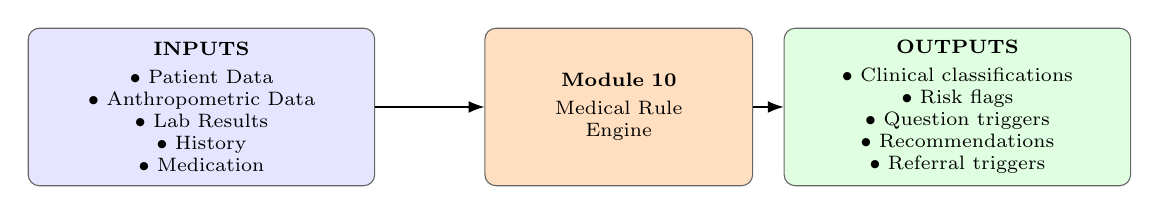
\begin{tikzpicture}[>=Latex]
\node[draw=black!60,rounded corners,fill=blue!10,minimum width=4.4cm,minimum height=2.0cm,align=center,font=\scriptsize,text width=4.15cm,inner sep=2pt] (io_in) at (0,0) {\textbf{\scriptsize INPUTS}\\[2pt]$\bullet$ Patient Data\\$\bullet$ Anthropometric Data\\$\bullet$ Lab Results\\$\bullet$ History\\$\bullet$ Medication};
\node[draw=black!60,rounded corners,fill=orange!25,minimum width=3.4cm,minimum height=2.0cm,align=center,font=\scriptsize,text width=3.15cm,inner sep=2pt] (io_p) at (5.3,0) {\textbf{Module 10}\\[2pt]Medical Rule\\Engine};
\node[draw=black!60,rounded corners,fill=green!12,minimum width=4.4cm,minimum height=2.0cm,align=center,font=\scriptsize,text width=4.15cm,inner sep=2pt] (io_out) at (9.6,0) {\textbf{\scriptsize OUTPUTS}\\[2pt]$\bullet$ Clinical classifications\\$\bullet$ Risk flags\\$\bullet$ Question triggers\\$\bullet$ Recommendations\\$\bullet$ Referral triggers};
\draw[-{Latex[length=2mm]}] (io_in.east)--(io_p.west);
\draw[-{Latex[length=2mm]}] (io_p.east)--(io_out.west);
\end{tikzpicture}
\end{adjustbox}
\end{center}
\end{frame}

\begin{frame}[t]{Module 10: Rule Engine / Medical Logic Engine}
\textcolor{black!55}{\scriptsize One value, traced through the engine}\\[2pt]
\begin{center}
\begin{adjustbox}{max width=0.96\linewidth,max height=0.62\textheight}
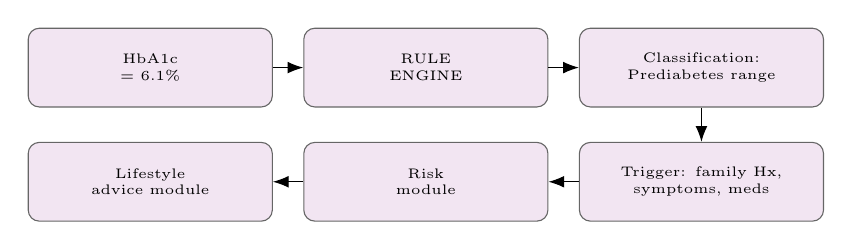
\begin{tikzpicture}[>=Latex]
\node[draw=black!60,rounded corners,fill=violet!10,minimum width=3.1cm,minimum height=1.0cm,align=center,font=\tiny,text width=2.85cm,inner sep=2pt] (s0) at (0.0,0.0) {HbA1c\\= 6.1\%};
\node[draw=black!60,rounded corners,fill=violet!10,minimum width=3.1cm,minimum height=1.0cm,align=center,font=\tiny,text width=2.85cm,inner sep=2pt] (s1) at (3.5,0.0) {RULE\\ENGINE};
\node[draw=black!60,rounded corners,fill=violet!10,minimum width=3.1cm,minimum height=1.0cm,align=center,font=\tiny,text width=2.85cm,inner sep=2pt] (s2) at (7.0,0.0) {Classification:\\Prediabetes range};
\node[draw=black!60,rounded corners,fill=violet!10,minimum width=3.1cm,minimum height=1.0cm,align=center,font=\tiny,text width=2.85cm,inner sep=2pt] (s3) at (7.0,-1.45) {Trigger: family Hx,\\symptoms, meds};
\node[draw=black!60,rounded corners,fill=violet!10,minimum width=3.1cm,minimum height=1.0cm,align=center,font=\tiny,text width=2.85cm,inner sep=2pt] (s4) at (3.5,-1.45) {Risk\\module};
\node[draw=black!60,rounded corners,fill=violet!10,minimum width=3.1cm,minimum height=1.0cm,align=center,font=\tiny,text width=2.85cm,inner sep=2pt] (s5) at (0.0,-1.45) {Lifestyle\\advice module};
\draw[-{Latex[length=2mm]}] (s0.east)--(s1.west);
\draw[-{Latex[length=2mm]}] (s1.east)--(s2.west);
\draw[-{Latex[length=2mm]}] (s2.south)--(s3.north);
\draw[-{Latex[length=2mm]}] (s3.west)--(s4.east);
\draw[-{Latex[length=2mm]}] (s4.west)--(s5.east);
\end{tikzpicture}
\end{adjustbox}
\end{center}
\end{frame}

\begin{frame}[t]{Module 11: Question Trigger Engine}
\textcolor{black!55}{\scriptsize Cluster 3 -- \textcolor{violet}{\textbf{Medical Intelligence Core}} (M10--M13) \\ Example 1 -- ALT elevated}\\[2pt]
\begin{itemize}
\scriptsize
\item Independent module -- users should not answer 80 questions at registration
\item An abnormal finding activates only the relevant question set
\item This is the module that makes the platform feel ``intelligent''
\end{itemize}
\vspace{4pt}
\begin{center}
\begin{adjustbox}{max width=0.96\linewidth,max height=0.62\textheight}
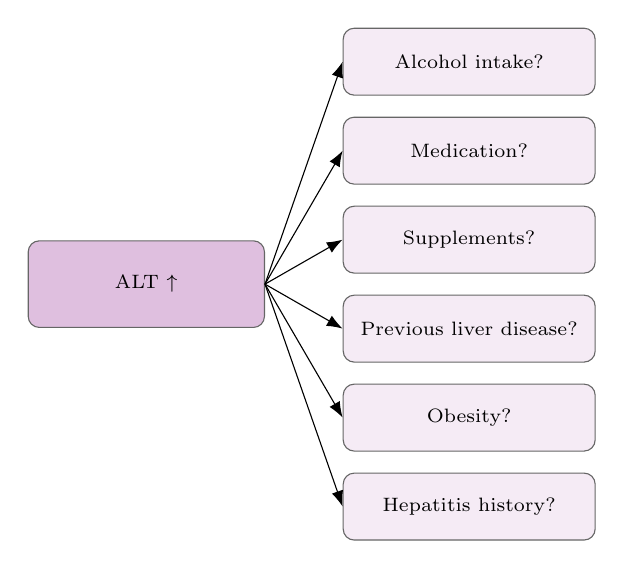
\begin{tikzpicture}[>=Latex]
\node[draw=black!60,rounded corners,fill=violet!25,minimum width=3.0cm,minimum height=1.1cm,align=center,font=\scriptsize,text width=2.75cm,inner sep=2pt] (q1c) at (0,-2.825) {ALT $\uparrow$};
\node[draw=black!60,rounded corners,fill=violet!8,minimum width=3.2cm,minimum height=0.85cm,align=center,font=\scriptsize,text width=2.95cm,inner sep=2pt] (q10) at (4.1,0) {Alcohol intake?};
\draw[-{Latex[length=2mm]}] (q1c.east)--(q10.west);
\node[draw=black!60,rounded corners,fill=violet!8,minimum width=3.2cm,minimum height=0.85cm,align=center,font=\scriptsize,text width=2.95cm,inner sep=2pt] (q11) at (4.1,-1.13) {Medication?};
\draw[-{Latex[length=2mm]}] (q1c.east)--(q11.west);
\node[draw=black!60,rounded corners,fill=violet!8,minimum width=3.2cm,minimum height=0.85cm,align=center,font=\scriptsize,text width=2.95cm,inner sep=2pt] (q12) at (4.1,-2.26) {Supplements?};
\draw[-{Latex[length=2mm]}] (q1c.east)--(q12.west);
\node[draw=black!60,rounded corners,fill=violet!8,minimum width=3.2cm,minimum height=0.85cm,align=center,font=\scriptsize,text width=2.95cm,inner sep=2pt] (q13) at (4.1,-3.3899999999999997) {Previous liver disease?};
\draw[-{Latex[length=2mm]}] (q1c.east)--(q13.west);
\node[draw=black!60,rounded corners,fill=violet!8,minimum width=3.2cm,minimum height=0.85cm,align=center,font=\scriptsize,text width=2.95cm,inner sep=2pt] (q14) at (4.1,-4.52) {Obesity?};
\draw[-{Latex[length=2mm]}] (q1c.east)--(q14.west);
\node[draw=black!60,rounded corners,fill=violet!8,minimum width=3.2cm,minimum height=0.85cm,align=center,font=\scriptsize,text width=2.95cm,inner sep=2pt] (q15) at (4.1,-5.6499999999999995) {Hepatitis history?};
\draw[-{Latex[length=2mm]}] (q1c.east)--(q15.west);
\end{tikzpicture}
\end{adjustbox}
\end{center}
\end{frame}

\begin{frame}[t]{Module 11: Question Trigger Engine}
\textcolor{black!55}{\scriptsize A second finding, a different question set}\\[2pt]
\begin{center}
\begin{adjustbox}{max width=0.96\linewidth,max height=0.62\textheight}
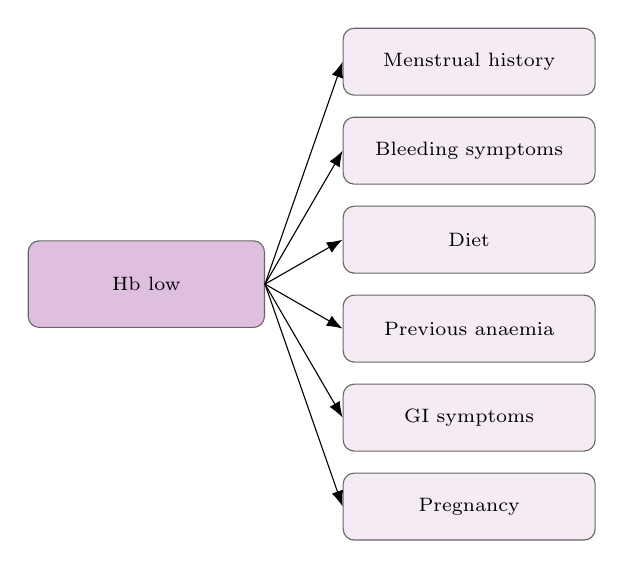
\begin{tikzpicture}[>=Latex]
\node[draw=black!60,rounded corners,fill=violet!25,minimum width=3.0cm,minimum height=1.1cm,align=center,font=\scriptsize,text width=2.75cm,inner sep=2pt] (q2c) at (0,-2.825) {Hb low};
\node[draw=black!60,rounded corners,fill=violet!8,minimum width=3.2cm,minimum height=0.85cm,align=center,font=\scriptsize,text width=2.95cm,inner sep=2pt] (q20) at (4.1,0) {Menstrual history};
\draw[-{Latex[length=2mm]}] (q2c.east)--(q20.west);
\node[draw=black!60,rounded corners,fill=violet!8,minimum width=3.2cm,minimum height=0.85cm,align=center,font=\scriptsize,text width=2.95cm,inner sep=2pt] (q21) at (4.1,-1.13) {Bleeding symptoms};
\draw[-{Latex[length=2mm]}] (q2c.east)--(q21.west);
\node[draw=black!60,rounded corners,fill=violet!8,minimum width=3.2cm,minimum height=0.85cm,align=center,font=\scriptsize,text width=2.95cm,inner sep=2pt] (q22) at (4.1,-2.26) {Diet};
\draw[-{Latex[length=2mm]}] (q2c.east)--(q22.west);
\node[draw=black!60,rounded corners,fill=violet!8,minimum width=3.2cm,minimum height=0.85cm,align=center,font=\scriptsize,text width=2.95cm,inner sep=2pt] (q23) at (4.1,-3.3899999999999997) {Previous anaemia};
\draw[-{Latex[length=2mm]}] (q2c.east)--(q23.west);
\node[draw=black!60,rounded corners,fill=violet!8,minimum width=3.2cm,minimum height=0.85cm,align=center,font=\scriptsize,text width=2.95cm,inner sep=2pt] (q24) at (4.1,-4.52) {GI symptoms};
\draw[-{Latex[length=2mm]}] (q2c.east)--(q24.west);
\node[draw=black!60,rounded corners,fill=violet!8,minimum width=3.2cm,minimum height=0.85cm,align=center,font=\scriptsize,text width=2.95cm,inner sep=2pt] (q25) at (4.1,-5.6499999999999995) {Pregnancy};
\draw[-{Latex[length=2mm]}] (q2c.east)--(q25.west);
\end{tikzpicture}
\end{adjustbox}
\end{center}
\end{frame}

\begin{frame}[t]{Module 12: Risk Stratification Engine}
\textcolor{black!55}{\scriptsize Cluster 3 -- \textcolor{violet}{\textbf{Medical Intelligence Core}} (M10--M13) \\ Many classification inputs converge into one risk output}\\[2pt]
\begin{itemize}
\scriptsize
\item Classification and risk must stay separate: ``LDL = high'' is a classification, not a risk score
\item Age + sex + smoking + BP + diabetes + cholesterol + history together may produce ``Cardiovascular risk = elevated''
\item Each calculator needs an ID, required variables, formula, exclusions, interpretation, version, source guideline
\end{itemize}
\vspace{4pt}
\begin{center}
\begin{adjustbox}{max width=0.96\linewidth,max height=0.62\textheight}
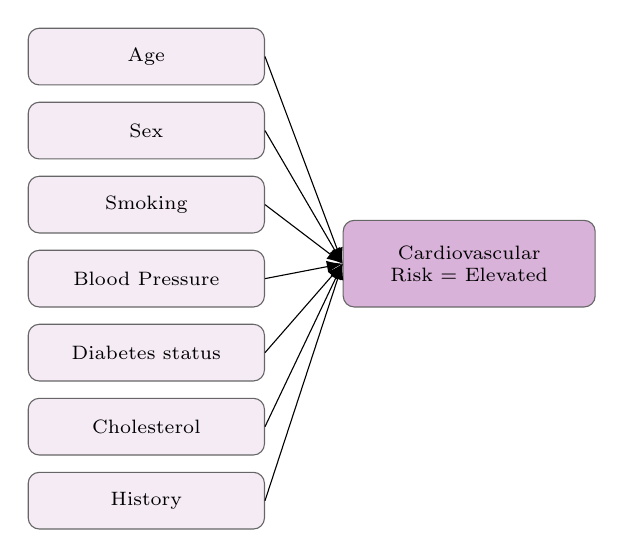
\begin{tikzpicture}[>=Latex]
\node[draw=black!60,rounded corners,fill=violet!8,minimum width=3.0cm,minimum height=0.72cm,align=center,font=\scriptsize,text width=2.75cm,inner sep=2pt] (hi0) at (0,0) {Age};
\node[draw=black!60,rounded corners,fill=violet!8,minimum width=3.0cm,minimum height=0.72cm,align=center,font=\scriptsize,text width=2.75cm,inner sep=2pt] (hi1) at (0,-0.94) {Sex};
\node[draw=black!60,rounded corners,fill=violet!8,minimum width=3.0cm,minimum height=0.72cm,align=center,font=\scriptsize,text width=2.75cm,inner sep=2pt] (hi2) at (0,-1.88) {Smoking};
\node[draw=black!60,rounded corners,fill=violet!8,minimum width=3.0cm,minimum height=0.72cm,align=center,font=\scriptsize,text width=2.75cm,inner sep=2pt] (hi3) at (0,-2.82) {Blood Pressure};
\node[draw=black!60,rounded corners,fill=violet!8,minimum width=3.0cm,minimum height=0.72cm,align=center,font=\scriptsize,text width=2.75cm,inner sep=2pt] (hi4) at (0,-3.76) {Diabetes status};
\node[draw=black!60,rounded corners,fill=violet!8,minimum width=3.0cm,minimum height=0.72cm,align=center,font=\scriptsize,text width=2.75cm,inner sep=2pt] (hi5) at (0,-4.699999999999999) {Cholesterol};
\node[draw=black!60,rounded corners,fill=violet!8,minimum width=3.0cm,minimum height=0.72cm,align=center,font=\scriptsize,text width=2.75cm,inner sep=2pt] (hi6) at (0,-5.639999999999999) {History};
\node[draw=black!60,rounded corners,fill=violet!30,minimum width=3.2cm,minimum height=1.1cm,align=center,font=\scriptsize,text width=2.95cm,inner sep=2pt] (hic) at (4.1,-2.63) {Cardiovascular\\Risk = Elevated};
\draw[-{Latex[length=2mm]}] (hi0.east)--(hic.west);
\draw[-{Latex[length=2mm]}] (hi1.east)--(hic.west);
\draw[-{Latex[length=2mm]}] (hi2.east)--(hic.west);
\draw[-{Latex[length=2mm]}] (hi3.east)--(hic.west);
\draw[-{Latex[length=2mm]}] (hi4.east)--(hic.west);
\draw[-{Latex[length=2mm]}] (hi5.east)--(hic.west);
\draw[-{Latex[length=2mm]}] (hi6.east)--(hic.west);
\end{tikzpicture}
\end{adjustbox}
\end{center}
\end{frame}

\begin{frame}[t]{Module 13: Red Flag / Escalation Module}
\textcolor{black!55}{\scriptsize Cluster 3 -- \textcolor{violet}{\textbf{Medical Intelligence Core}} (M10--M13) \\ Five-stage escalation ladder}\\[2pt]
\begin{itemize}
\scriptsize
\item Separates Normal wellness $\to$ Monitor $\to$ Medical review $\to$ Urgent review $\to$ Emergency advice
\item Red flags are centrally controlled and versioned, never scattered across screens
\end{itemize}
\vspace{4pt}
\begin{center}
\begin{adjustbox}{max width=0.96\linewidth,max height=0.62\textheight}
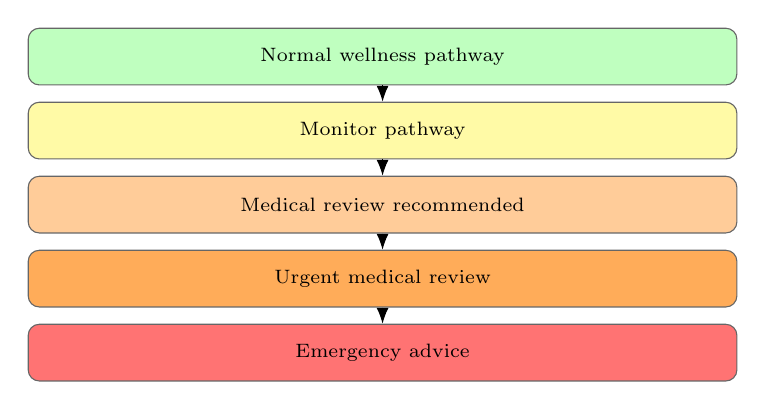
\begin{tikzpicture}[>=Latex]
\node[draw=black!60,rounded corners,fill=green!25,minimum width=9.0cm,minimum height=0.72cm,align=center,font=\scriptsize,text width=8.75cm,inner sep=2pt] (lv0) at (0,0) {Normal wellness pathway};
\node[draw=black!60,rounded corners,fill=yellow!35,minimum width=9.0cm,minimum height=0.72cm,align=center,font=\scriptsize,text width=8.75cm,inner sep=2pt] (lv1) at (0,-0.94) {Monitor pathway};
\node[draw=black!60,rounded corners,fill=orange!40,minimum width=9.0cm,minimum height=0.72cm,align=center,font=\scriptsize,text width=8.75cm,inner sep=2pt] (lv2) at (0,-1.88) {Medical review recommended};
\node[draw=black!60,rounded corners,fill=orange!65,minimum width=9.0cm,minimum height=0.72cm,align=center,font=\scriptsize,text width=8.75cm,inner sep=2pt] (lv3) at (0,-2.82) {Urgent medical review};
\node[draw=black!60,rounded corners,fill=red!55,minimum width=9.0cm,minimum height=0.72cm,align=center,font=\scriptsize,text width=8.75cm,inner sep=2pt] (lv4) at (0,-3.76) {Emergency advice};
\draw[-{Latex[length=2mm]}] (lv0.south)--(lv1.north);
\draw[-{Latex[length=2mm]}] (lv1.south)--(lv2.north);
\draw[-{Latex[length=2mm]}] (lv2.south)--(lv3.north);
\draw[-{Latex[length=2mm]}] (lv3.south)--(lv4.north);
\end{tikzpicture}
\end{adjustbox}
\end{center}
\end{frame}

\begin{frame}[t]{Module 13: Red Flag / Escalation Module}
\textcolor{black!55}{\scriptsize One gate, two possible outcomes}\\[2pt]
\begin{center}
\begin{adjustbox}{max width=0.96\linewidth,max height=0.62\textheight}
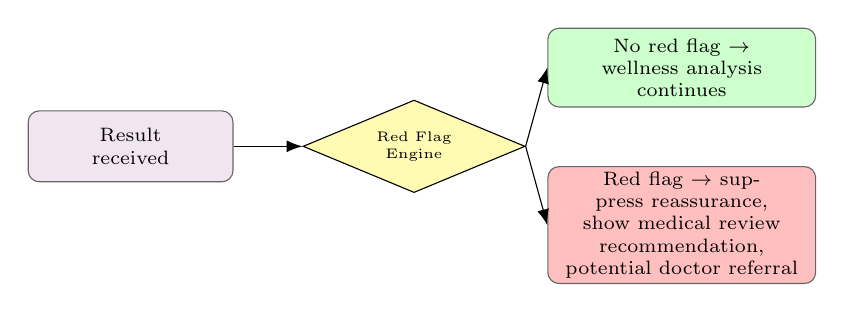
\begin{tikzpicture}[>=Latex]
\node[draw=black!60,rounded corners,fill=violet!10,minimum width=2.6cm,minimum height=0.9cm,align=center,font=\scriptsize,text width=2.35cm,inner sep=2pt] (rf1) at (0,0) {Result\\received};
\node[draw,diamond,aspect=2.4,fill=yellow!30,align=center,font=\tiny,text width=1.7000000000000002cm,inner sep=1pt] (rf2) at (3.6,0) {Red Flag\\Engine};
\draw[-{Latex[length=2mm]}] (rf1.east)--(rf2.west);
\node[draw=black!60,rounded corners,fill=green!20,minimum width=3.4cm,minimum height=1.0cm,align=center,font=\scriptsize,text width=3.15cm,inner sep=2pt] (rf3) at (7.0,1.0) {No red flag $\to$\\wellness analysis\\continues};
\node[draw=black!60,rounded corners,fill=red!25,minimum width=3.4cm,minimum height=1.2cm,align=center,font=\scriptsize,text width=3.15cm,inner sep=2pt] (rf4) at (7.0,-1.0) {Red flag $\to$ suppress reassurance,\\show medical review recommendation,\\potential doctor referral};
\draw[-{Latex[length=2mm]}] (rf2.east)--(rf3.west);
\draw[-{Latex[length=2mm]}] (rf2.east)--(rf4.west);
\end{tikzpicture}
\end{adjustbox}
\end{center}
\end{frame}

\section{Cluster 4 -- Interpretation \& Reporting (M14--M19)}

\begin{frame}[t]{Module 14: Health Domain Analysis Module}
\textcolor{black!55}{\scriptsize Cluster 4 -- \textcolor{orange}{\textbf{Interpretation \& Reporting}} (M14--M19) \\ Eleven interpretable health domains}\\[2pt]
\begin{itemize}
\scriptsize
\item Combines $\sim$40 individual tests into interpretable domains rather than a raw list
\item Metabolic, cardiovascular, glycaemic, lipid, kidney, liver, haematological, nutritional, thyroid, inflammatory, anthropometric health
\item Makes the report far easier for patients to understand
\end{itemize}
\vspace{4pt}
\begin{center}
\begin{adjustbox}{max width=0.96\linewidth,max height=0.62\textheight}
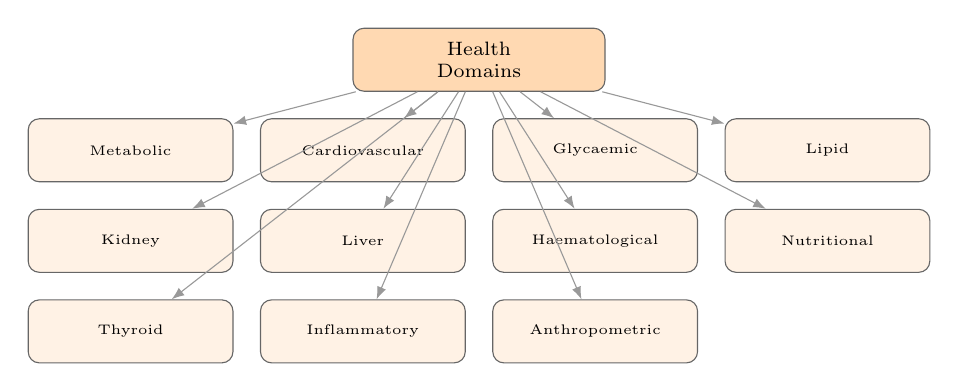
\begin{tikzpicture}[>=Latex]
\node[draw=black!60,rounded corners,fill=orange!10,minimum width=2.6cm,minimum height=0.8cm,align=center,font=\tiny,text width=2.35cm,inner sep=2pt] (g0) at (0.0,0.0) {Metabolic};
\node[draw=black!60,rounded corners,fill=orange!10,minimum width=2.6cm,minimum height=0.8cm,align=center,font=\tiny,text width=2.35cm,inner sep=2pt] (g1) at (2.95,0.0) {Cardiovascular};
\node[draw=black!60,rounded corners,fill=orange!10,minimum width=2.6cm,minimum height=0.8cm,align=center,font=\tiny,text width=2.35cm,inner sep=2pt] (g2) at (5.9,0.0) {Glycaemic};
\node[draw=black!60,rounded corners,fill=orange!10,minimum width=2.6cm,minimum height=0.8cm,align=center,font=\tiny,text width=2.35cm,inner sep=2pt] (g3) at (8.850000000000001,0.0) {Lipid};
\node[draw=black!60,rounded corners,fill=orange!10,minimum width=2.6cm,minimum height=0.8cm,align=center,font=\tiny,text width=2.35cm,inner sep=2pt] (g4) at (0.0,-1.15) {Kidney};
\node[draw=black!60,rounded corners,fill=orange!10,minimum width=2.6cm,minimum height=0.8cm,align=center,font=\tiny,text width=2.35cm,inner sep=2pt] (g5) at (2.95,-1.15) {Liver};
\node[draw=black!60,rounded corners,fill=orange!10,minimum width=2.6cm,minimum height=0.8cm,align=center,font=\tiny,text width=2.35cm,inner sep=2pt] (g6) at (5.9,-1.15) {Haematological};
\node[draw=black!60,rounded corners,fill=orange!10,minimum width=2.6cm,minimum height=0.8cm,align=center,font=\tiny,text width=2.35cm,inner sep=2pt] (g7) at (8.850000000000001,-1.15) {Nutritional};
\node[draw=black!60,rounded corners,fill=orange!10,minimum width=2.6cm,minimum height=0.8cm,align=center,font=\tiny,text width=2.35cm,inner sep=2pt] (g8) at (0.0,-2.3) {Thyroid};
\node[draw=black!60,rounded corners,fill=orange!10,minimum width=2.6cm,minimum height=0.8cm,align=center,font=\tiny,text width=2.35cm,inner sep=2pt] (g9) at (2.95,-2.3) {Inflammatory};
\node[draw=black!60,rounded corners,fill=orange!10,minimum width=2.6cm,minimum height=0.8cm,align=center,font=\tiny,text width=2.35cm,inner sep=2pt] (g10) at (5.9,-2.3) {Anthropometric};
\node[draw=black!60,rounded corners,fill=orange!30,minimum width=3.2cm,minimum height=0.8cm,align=center,font=\scriptsize,text width=2.95cm,inner sep=2pt] (gc) at (4.425000000000001,1.15) {Health\\Domains};
\draw[-{Latex[length=1.6mm]},black!40] (gc)--(g0);
\draw[-{Latex[length=1.6mm]},black!40] (gc)--(g1);
\draw[-{Latex[length=1.6mm]},black!40] (gc)--(g2);
\draw[-{Latex[length=1.6mm]},black!40] (gc)--(g3);
\draw[-{Latex[length=1.6mm]},black!40] (gc)--(g4);
\draw[-{Latex[length=1.6mm]},black!40] (gc)--(g5);
\draw[-{Latex[length=1.6mm]},black!40] (gc)--(g6);
\draw[-{Latex[length=1.6mm]},black!40] (gc)--(g7);
\draw[-{Latex[length=1.6mm]},black!40] (gc)--(g8);
\draw[-{Latex[length=1.6mm]},black!40] (gc)--(g9);
\draw[-{Latex[length=1.6mm]},black!40] (gc)--(g10);
\end{tikzpicture}
\end{adjustbox}
\end{center}
\end{frame}

\begin{frame}[t]{Module 14: Health Domain Analysis Module}
\textcolor{black!55}{\scriptsize Eight parameters, one domain interpretation}\\[2pt]
\begin{center}
\begin{adjustbox}{max width=0.96\linewidth,max height=0.62\textheight}
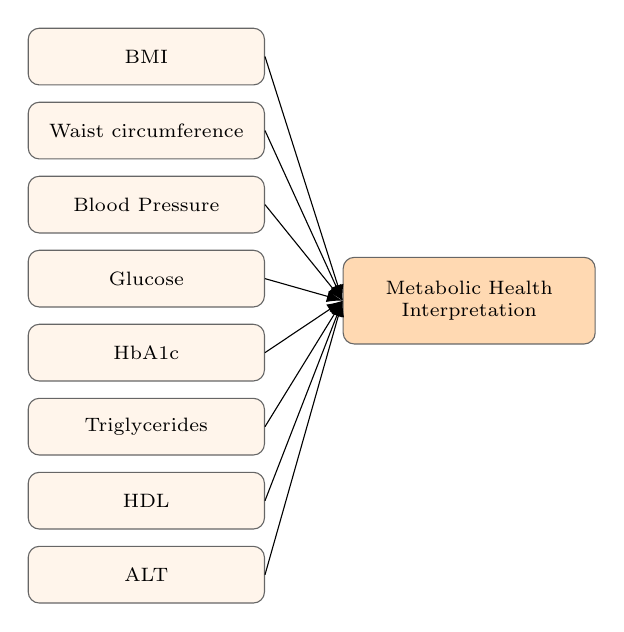
\begin{tikzpicture}[>=Latex]
\node[draw=black!60,rounded corners,fill=orange!8,minimum width=3.0cm,minimum height=0.72cm,align=center,font=\scriptsize,text width=2.75cm,inner sep=2pt] (mh0) at (0,0) {BMI};
\node[draw=black!60,rounded corners,fill=orange!8,minimum width=3.0cm,minimum height=0.72cm,align=center,font=\scriptsize,text width=2.75cm,inner sep=2pt] (mh1) at (0,-0.94) {Waist circumference};
\node[draw=black!60,rounded corners,fill=orange!8,minimum width=3.0cm,minimum height=0.72cm,align=center,font=\scriptsize,text width=2.75cm,inner sep=2pt] (mh2) at (0,-1.88) {Blood Pressure};
\node[draw=black!60,rounded corners,fill=orange!8,minimum width=3.0cm,minimum height=0.72cm,align=center,font=\scriptsize,text width=2.75cm,inner sep=2pt] (mh3) at (0,-2.82) {Glucose};
\node[draw=black!60,rounded corners,fill=orange!8,minimum width=3.0cm,minimum height=0.72cm,align=center,font=\scriptsize,text width=2.75cm,inner sep=2pt] (mh4) at (0,-3.76) {HbA1c};
\node[draw=black!60,rounded corners,fill=orange!8,minimum width=3.0cm,minimum height=0.72cm,align=center,font=\scriptsize,text width=2.75cm,inner sep=2pt] (mh5) at (0,-4.699999999999999) {Triglycerides};
\node[draw=black!60,rounded corners,fill=orange!8,minimum width=3.0cm,minimum height=0.72cm,align=center,font=\scriptsize,text width=2.75cm,inner sep=2pt] (mh6) at (0,-5.639999999999999) {HDL};
\node[draw=black!60,rounded corners,fill=orange!8,minimum width=3.0cm,minimum height=0.72cm,align=center,font=\scriptsize,text width=2.75cm,inner sep=2pt] (mh7) at (0,-6.579999999999998) {ALT};
\node[draw=black!60,rounded corners,fill=orange!30,minimum width=3.2cm,minimum height=1.1cm,align=center,font=\scriptsize,text width=2.95cm,inner sep=2pt] (mhc) at (4.1,-3.0999999999999996) {Metabolic Health\\Interpretation};
\draw[-{Latex[length=2mm]}] (mh0.east)--(mhc.west);
\draw[-{Latex[length=2mm]}] (mh1.east)--(mhc.west);
\draw[-{Latex[length=2mm]}] (mh2.east)--(mhc.west);
\draw[-{Latex[length=2mm]}] (mh3.east)--(mhc.west);
\draw[-{Latex[length=2mm]}] (mh4.east)--(mhc.west);
\draw[-{Latex[length=2mm]}] (mh5.east)--(mhc.west);
\draw[-{Latex[length=2mm]}] (mh6.east)--(mhc.west);
\draw[-{Latex[length=2mm]}] (mh7.east)--(mhc.west);
\end{tikzpicture}
\end{adjustbox}
\end{center}
\end{frame}

\begin{frame}[t]{Module 15: Recommendation Engine}
\textcolor{black!55}{\scriptsize Cluster 4 -- \textcolor{orange}{\textbf{Interpretation \& Reporting}} (M14--M19) \\ One finding combination, seven candidate recommendations}\\[2pt]
\begin{itemize}
\scriptsize
\item Recommendations are separate from classifications -- one classification can trigger several recommendations
\item Recommendations use codes (e.g. \texttt{REC\_DIET\_001}) instead of hard-coded text
\end{itemize}
\vspace{4pt}
\begin{center}
\begin{adjustbox}{max width=0.96\linewidth,max height=0.62\textheight}
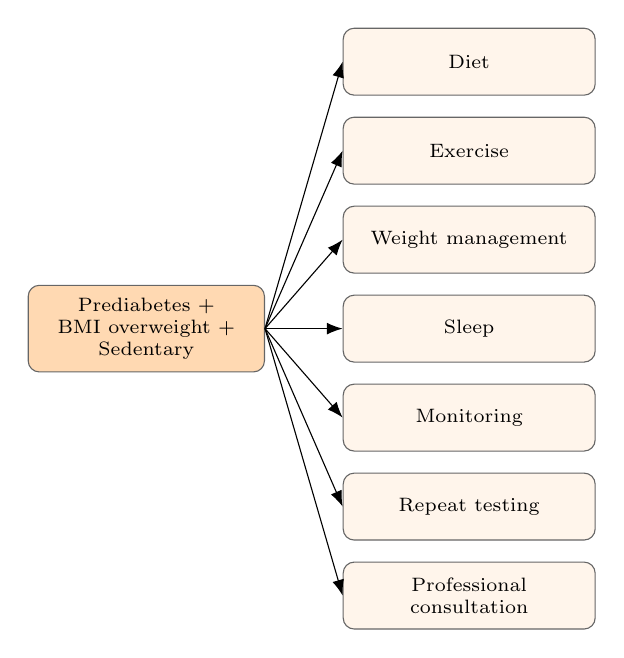
\begin{tikzpicture}[>=Latex]
\node[draw=black!60,rounded corners,fill=orange!30,minimum width=3.0cm,minimum height=1.1cm,align=center,font=\scriptsize,text width=2.75cm,inner sep=2pt] (hoc) at (0,-3.3900000000000006) {Prediabetes +\\BMI overweight +\\Sedentary};
\node[draw=black!60,rounded corners,fill=orange!8,minimum width=3.2cm,minimum height=0.85cm,align=center,font=\scriptsize,text width=2.95cm,inner sep=2pt] (ho0) at (4.1,0) {Diet};
\draw[-{Latex[length=2mm]}] (hoc.east)--(ho0.west);
\node[draw=black!60,rounded corners,fill=orange!8,minimum width=3.2cm,minimum height=0.85cm,align=center,font=\scriptsize,text width=2.95cm,inner sep=2pt] (ho1) at (4.1,-1.13) {Exercise};
\draw[-{Latex[length=2mm]}] (hoc.east)--(ho1.west);
\node[draw=black!60,rounded corners,fill=orange!8,minimum width=3.2cm,minimum height=0.85cm,align=center,font=\scriptsize,text width=2.95cm,inner sep=2pt] (ho2) at (4.1,-2.26) {Weight management};
\draw[-{Latex[length=2mm]}] (hoc.east)--(ho2.west);
\node[draw=black!60,rounded corners,fill=orange!8,minimum width=3.2cm,minimum height=0.85cm,align=center,font=\scriptsize,text width=2.95cm,inner sep=2pt] (ho3) at (4.1,-3.3899999999999997) {Sleep};
\draw[-{Latex[length=2mm]}] (hoc.east)--(ho3.west);
\node[draw=black!60,rounded corners,fill=orange!8,minimum width=3.2cm,minimum height=0.85cm,align=center,font=\scriptsize,text width=2.95cm,inner sep=2pt] (ho4) at (4.1,-4.52) {Monitoring};
\draw[-{Latex[length=2mm]}] (hoc.east)--(ho4.west);
\node[draw=black!60,rounded corners,fill=orange!8,minimum width=3.2cm,minimum height=0.85cm,align=center,font=\scriptsize,text width=2.95cm,inner sep=2pt] (ho5) at (4.1,-5.6499999999999995) {Repeat testing};
\draw[-{Latex[length=2mm]}] (hoc.east)--(ho5.west);
\node[draw=black!60,rounded corners,fill=orange!8,minimum width=3.2cm,minimum height=0.85cm,align=center,font=\scriptsize,text width=2.95cm,inner sep=2pt] (ho6) at (4.1,-6.779999999999999) {Professional consultation};
\draw[-{Latex[length=2mm]}] (hoc.east)--(ho6.west);
\end{tikzpicture}
\end{adjustbox}
\end{center}
\end{frame}

\begin{frame}[t]{Module 16: Explanation / Health Education Library}
\textcolor{black!55}{\scriptsize Cluster 4 -- \textcolor{orange}{\textbf{Interpretation \& Reporting}} (M14--M19) \\ Recommendation Engine calls the education library}\\[2pt]
\begin{itemize}
\scriptsize
\item A dedicated content library so the platform can explain \emph{why} advice is given
\item The Recommendation Engine calls these entries -- doctors can update wording without touching code
\end{itemize}
\vspace{4pt}
\begin{center}
\begin{adjustbox}{max width=0.96\linewidth,max height=0.62\textheight}
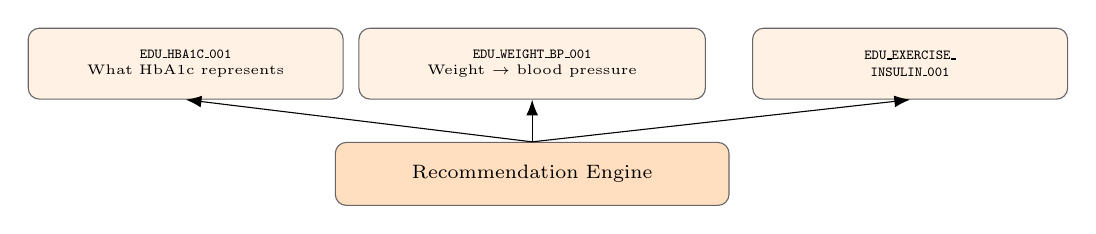
\begin{tikzpicture}[>=Latex]
\node[draw=black!60,rounded corners,fill=orange!10,minimum width=4.0cm,minimum height=0.9cm,align=center,font=\tiny,text width=3.75cm,inner sep=2pt] (e1) at (0,0.7) {\texttt{EDU\_HBA1C\_001}\\What HbA1c represents};
\node[draw=black!60,rounded corners,fill=orange!10,minimum width=4.4cm,minimum height=0.9cm,align=center,font=\tiny,text width=4.15cm,inner sep=2pt] (e2) at (4.4,0.7) {\texttt{EDU\_WEIGHT\_BP\_001}\\Weight $\to$ blood pressure};
\node[draw=black!60,rounded corners,fill=orange!10,minimum width=4.0cm,minimum height=0.9cm,align=center,font=\tiny,text width=3.75cm,inner sep=2pt] (e3) at (9.2,0.7) {\texttt{EDU\_EXERCISE\_}\\\texttt{INSULIN\_001}};
\node[draw=black!60,rounded corners,fill=orange!25,minimum width=5.0cm,minimum height=0.8cm,align=center,font=\scriptsize,text width=4.75cm,inner sep=2pt] (e4) at (4.4,-0.7) {Recommendation Engine};
\draw[-{Latex[length=2mm]}] (e4.north)--(e1.south);
\draw[-{Latex[length=2mm]}] (e4.north)--(e2.south);
\draw[-{Latex[length=2mm]}] (e4.north)--(e3.south);
\end{tikzpicture}
\end{adjustbox}
\end{center}
\end{frame}

\begin{frame}[t]{Module 17: Trend \& Longitudinal Health Module}
\textcolor{black!55}{\scriptsize Cluster 4 -- \textcolor{orange}{\textbf{Interpretation \& Reporting}} (M14--M19) \\ A falling HbA1c series classified as Improving}\\[2pt]
\begin{itemize}
\scriptsize
\item Every parameter is stored longitudinally, not just archived as a PDF
\item Computes absolute/percentage change, direction, rate of change, persistent/new/resolved abnormality
\end{itemize}
\vspace{4pt}
\begin{center}
\begin{adjustbox}{max width=0.96\linewidth,max height=0.62\textheight}
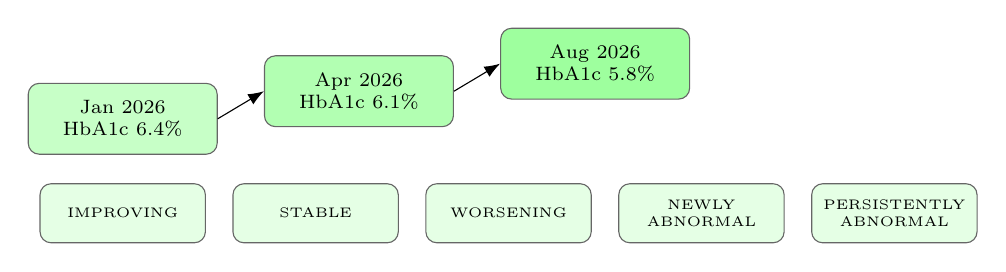
\begin{tikzpicture}[>=Latex]
\node[draw=black!60,rounded corners,fill=green!22,minimum width=2.4cm,minimum height=0.9cm,align=center,font=\scriptsize,text width=2.15cm,inner sep=2pt] (t1) at (0,0.2) {Jan 2026\\HbA1c 6.4\%};
\node[draw=black!60,rounded corners,fill=green!30,minimum width=2.4cm,minimum height=0.9cm,align=center,font=\scriptsize,text width=2.15cm,inner sep=2pt] (t2) at (3.0,0.55) {Apr 2026\\HbA1c 6.1\%};
\node[draw=black!60,rounded corners,fill=green!38,minimum width=2.4cm,minimum height=0.9cm,align=center,font=\scriptsize,text width=2.15cm,inner sep=2pt] (t3) at (6.0,0.9) {Aug 2026\\HbA1c 5.8\%};
\draw[-{Latex[length=2mm]}] (t1.east)--(t2.west);
\draw[-{Latex[length=2mm]}] (t2.east)--(t3.west);
\begin{scope}[shift={(0,-1.0)}]
\node[draw=black!60,rounded corners,fill=green!10,minimum width=2.1cm,minimum height=0.75cm,align=center,font=\tiny,text width=1.85cm,inner sep=2pt] (tc0) at (0.0,0.0) {IMPROVING};
\node[draw=black!60,rounded corners,fill=green!10,minimum width=2.1cm,minimum height=0.75cm,align=center,font=\tiny,text width=1.85cm,inner sep=2pt] (tc1) at (2.45,0.0) {STABLE};
\node[draw=black!60,rounded corners,fill=green!10,minimum width=2.1cm,minimum height=0.75cm,align=center,font=\tiny,text width=1.85cm,inner sep=2pt] (tc2) at (4.9,0.0) {WORSENING};
\node[draw=black!60,rounded corners,fill=green!10,minimum width=2.1cm,minimum height=0.75cm,align=center,font=\tiny,text width=1.85cm,inner sep=2pt] (tc3) at (7.3500000000000005,0.0) {NEWLY\\ABNORMAL};
\node[draw=black!60,rounded corners,fill=green!10,minimum width=2.1cm,minimum height=0.75cm,align=center,font=\tiny,text width=1.85cm,inner sep=2pt] (tc4) at (9.8,0.0) {PERSISTENTLY\\ABNORMAL};
\end{scope}
\end{tikzpicture}
\end{adjustbox}
\end{center}
\end{frame}

\begin{frame}[t]{Module 18: Health Score Module}
\textcolor{black!55}{\scriptsize Cluster 4 -- \textcolor{orange}{\textbf{Interpretation \& Reporting}} (M14--M19) \\ A communication layer, never a substitute for classification}\\[2pt]
\begin{itemize}
\scriptsize
\item If used, kept separate from clinical classifications: metabolic, cardiovascular wellness, lifestyle, overall profile scores
\item \textbf{Clinical result $\neq$ health score} -- the score communicates, it does not replace medical classification
\end{itemize}
\vspace{4pt}
\begin{center}
\begin{adjustbox}{max width=0.96\linewidth,max height=0.62\textheight}
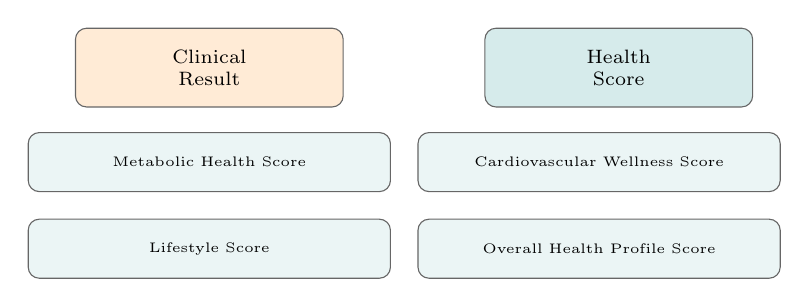
\begin{tikzpicture}[>=Latex]
\node[draw=black!60,rounded corners,fill=orange!16,minimum width=3.4cm,minimum height=1.0cm,align=center,font=\scriptsize,text width=3.15cm,inner sep=2pt] (hs1) at (0,0) {Clinical\\Result};
\node[draw=white,rounded corners,fill=white,minimum width=0.8cm,minimum height=1.0cm,align=center,font=\Large,text width=0.6cm,inner sep=2pt] (hsne) at (3.9,0) {$\neq$};
\node[draw=black!60,rounded corners,fill=teal!16,minimum width=3.4cm,minimum height=1.0cm,align=center,font=\scriptsize,text width=3.15cm,inner sep=2pt] (hs2) at (5.2,0) {Health\\Score};
\begin{scope}[shift={(0,-1.2)}]
\node[draw=black!60,rounded corners,fill=teal!8,minimum width=4.6cm,minimum height=0.75cm,align=center,font=\tiny,text width=4.35cm,inner sep=2pt] (hst0) at (0.0,0.0) {Metabolic Health Score};
\node[draw=black!60,rounded corners,fill=teal!8,minimum width=4.6cm,minimum height=0.75cm,align=center,font=\tiny,text width=4.35cm,inner sep=2pt] (hst1) at (4.949999999999999,0.0) {Cardiovascular Wellness Score};
\node[draw=black!60,rounded corners,fill=teal!8,minimum width=4.6cm,minimum height=0.75cm,align=center,font=\tiny,text width=4.35cm,inner sep=2pt] (hst2) at (0.0,-1.1) {Lifestyle Score};
\node[draw=black!60,rounded corners,fill=teal!8,minimum width=4.6cm,minimum height=0.75cm,align=center,font=\tiny,text width=4.35cm,inner sep=2pt] (hst3) at (4.949999999999999,-1.1) {Overall Health Profile Score};
\end{scope}
\end{tikzpicture}
\end{adjustbox}
\end{center}
\end{frame}

\begin{frame}[t]{Module 19: Report Generation Module}
\textcolor{black!55}{\scriptsize Cluster 4 -- \textcolor{orange}{\textbf{Interpretation \& Reporting}} (M14--M19) \\ Eight inputs assembled into a twelve-section report}\\[2pt]
\begin{itemize}
\scriptsize
\item Assembles every other module's output into one report
\item Twelve-section structure: summary, findings, anthropometrics, results, domains, trends, risk factors, attention areas, recommendations, rationale, monitoring, referral
\end{itemize}
\vspace{4pt}
\begin{center}
\begin{adjustbox}{max width=0.96\linewidth,max height=0.62\textheight}
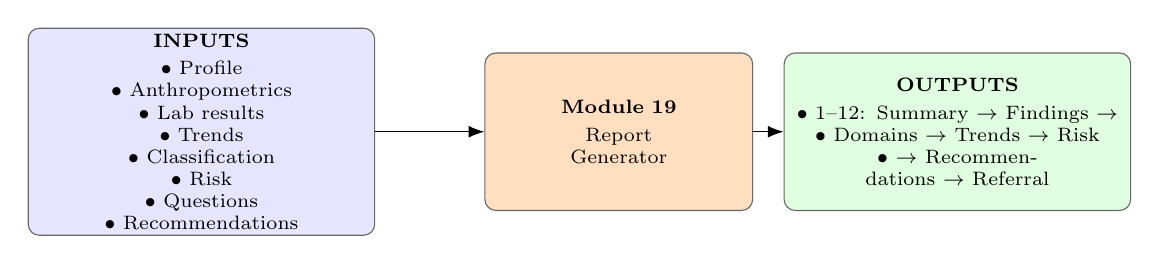
\begin{tikzpicture}[>=Latex]
\node[draw=black!60,rounded corners,fill=blue!10,minimum width=4.4cm,minimum height=2.0cm,align=center,font=\scriptsize,text width=4.15cm,inner sep=2pt] (io_in) at (0,0) {\textbf{\scriptsize INPUTS}\\[2pt]$\bullet$ Profile\\$\bullet$ Anthropometrics\\$\bullet$ Lab results\\$\bullet$ Trends\\$\bullet$ Classification\\$\bullet$ Risk\\$\bullet$ Questions\\$\bullet$ Recommendations};
\node[draw=black!60,rounded corners,fill=orange!25,minimum width=3.4cm,minimum height=2.0cm,align=center,font=\scriptsize,text width=3.15cm,inner sep=2pt] (io_p) at (5.3,0) {\textbf{Module 19}\\[2pt]Report\\Generator};
\node[draw=black!60,rounded corners,fill=green!12,minimum width=4.4cm,minimum height=2.0cm,align=center,font=\scriptsize,text width=4.15cm,inner sep=2pt] (io_out) at (9.6,0) {\textbf{\scriptsize OUTPUTS}\\[2pt]$\bullet$ 1--12: Summary $\to$ Findings $\to$\\$\bullet$ Domains $\to$ Trends $\to$ Risk\\$\bullet$ $\to$ Recommendations $\to$ Referral};
\draw[-{Latex[length=2mm]}] (io_in.east)--(io_p.west);
\draw[-{Latex[length=2mm]}] (io_p.east)--(io_out.west);
\end{tikzpicture}
\end{adjustbox}
\end{center}
\end{frame}

\section{Cluster 5 -- Engagement (M20--M21)}

\begin{frame}[t]{Module 20: Referral \& Professional Network Module}
\textcolor{black!55}{\scriptsize Cluster 5 -- \textcolor{green!60!black}{\textbf{Engagement}} (M20--M21) \\ Rule-triggered referral, not advertising}\\[2pt]
\begin{itemize}
\scriptsize
\item Later supports doctor, dietitian, physiotherapist, pharmacist, fitness professional, other wellness professionals
\item Triggered by medical logic, not arbitrary advertising
\end{itemize}
\vspace{4pt}
\begin{center}
\begin{adjustbox}{max width=0.96\linewidth,max height=0.62\textheight}
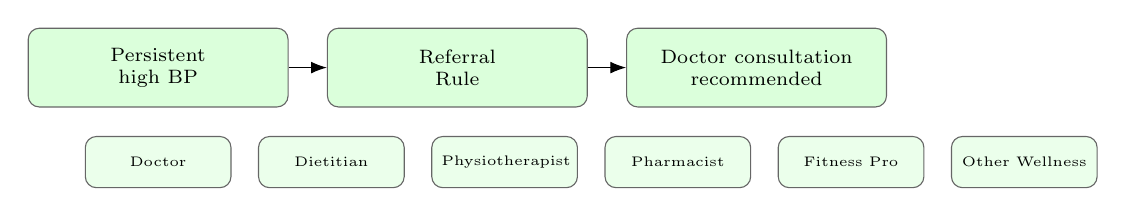
\begin{tikzpicture}[>=Latex]
\node[draw=black!60,rounded corners,fill=green!14,minimum width=3.3cm,minimum height=1.0cm,align=center,font=\scriptsize,text width=3.05cm,inner sep=2pt] (h0) at (0,0) {Persistent\\high BP};
\node[draw=black!60,rounded corners,fill=green!14,minimum width=3.3cm,minimum height=1.0cm,align=center,font=\scriptsize,text width=3.05cm,inner sep=2pt] (h1) at (3.8,0) {Referral\\Rule};
\node[draw=black!60,rounded corners,fill=green!14,minimum width=3.3cm,minimum height=1.0cm,align=center,font=\scriptsize,text width=3.05cm,inner sep=2pt] (h2) at (7.6,0) {Doctor consultation\\recommended};
\draw[-{Latex[length=2mm]}] (h0.east)--(h1.west);
\draw[-{Latex[length=2mm]}] (h1.east)--(h2.west);
\begin{scope}[shift={(0,-1.2)}]
\node[draw=black!60,rounded corners,fill=green!8,minimum width=1.85cm,minimum height=0.65cm,align=center,font=\tiny,text width=1.6cm,inner sep=2pt] (pn0) at (0.0,0.0) {Doctor};
\node[draw=black!60,rounded corners,fill=green!8,minimum width=1.85cm,minimum height=0.65cm,align=center,font=\tiny,text width=1.6cm,inner sep=2pt] (pn1) at (2.2,0.0) {Dietitian};
\node[draw=black!60,rounded corners,fill=green!8,minimum width=1.85cm,minimum height=0.65cm,align=center,font=\tiny,text width=1.6cm,inner sep=2pt] (pn2) at (4.4,0.0) {Physiotherapist};
\node[draw=black!60,rounded corners,fill=green!8,minimum width=1.85cm,minimum height=0.65cm,align=center,font=\tiny,text width=1.6cm,inner sep=2pt] (pn3) at (6.6000000000000005,0.0) {Pharmacist};
\node[draw=black!60,rounded corners,fill=green!8,minimum width=1.85cm,minimum height=0.65cm,align=center,font=\tiny,text width=1.6cm,inner sep=2pt] (pn4) at (8.8,0.0) {Fitness Pro};
\node[draw=black!60,rounded corners,fill=green!8,minimum width=1.85cm,minimum height=0.65cm,align=center,font=\tiny,text width=1.6cm,inner sep=2pt] (pn5) at (11.0,0.0) {Other Wellness};
\end{scope}
\end{tikzpicture}
\end{adjustbox}
\end{center}
\end{frame}

\begin{frame}[t]{Module 21: Notification \& Follow-Up Module}
\textcolor{black!55}{\scriptsize Cluster 5 -- \textcolor{green!60!black}{\textbf{Engagement}} (M20--M21) \\ Six example follow-up triggers}\\[2pt]
\begin{itemize}
\scriptsize
\item Creates longitudinal engagement instead of a one-time blood-report service
\end{itemize}
\vspace{4pt}
\begin{center}
\begin{adjustbox}{max width=0.96\linewidth,max height=0.62\textheight}
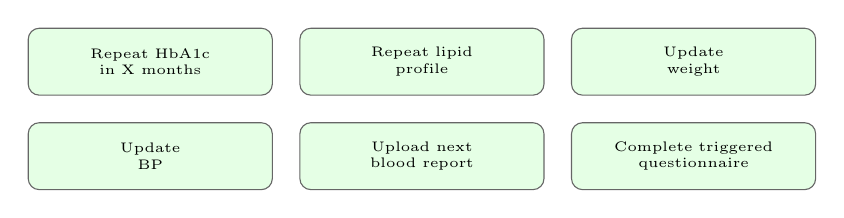
\begin{tikzpicture}[>=Latex]
\node[draw=black!60,rounded corners,fill=green!10,minimum width=3.1cm,minimum height=0.85cm,align=center,font=\tiny,text width=2.85cm,inner sep=2pt] (g0) at (0.0,0.0) {Repeat HbA1c\\in X months};
\node[draw=black!60,rounded corners,fill=green!10,minimum width=3.1cm,minimum height=0.85cm,align=center,font=\tiny,text width=2.85cm,inner sep=2pt] (g1) at (3.45,0.0) {Repeat lipid\\profile};
\node[draw=black!60,rounded corners,fill=green!10,minimum width=3.1cm,minimum height=0.85cm,align=center,font=\tiny,text width=2.85cm,inner sep=2pt] (g2) at (6.9,0.0) {Update\\weight};
\node[draw=black!60,rounded corners,fill=green!10,minimum width=3.1cm,minimum height=0.85cm,align=center,font=\tiny,text width=2.85cm,inner sep=2pt] (g3) at (0.0,-1.2) {Update\\BP};
\node[draw=black!60,rounded corners,fill=green!10,minimum width=3.1cm,minimum height=0.85cm,align=center,font=\tiny,text width=2.85cm,inner sep=2pt] (g4) at (3.45,-1.2) {Upload next\\blood report};
\node[draw=black!60,rounded corners,fill=green!10,minimum width=3.1cm,minimum height=0.85cm,align=center,font=\tiny,text width=2.85cm,inner sep=2pt] (g5) at (6.9,-1.2) {Complete triggered\\questionnaire};
\end{tikzpicture}
\end{adjustbox}
\end{center}
\end{frame}

\section{Cluster 6 -- Platform Governance (M22--M26)}

\begin{frame}[t]{Module 22: Medical Knowledge Management / Admin Module}
\textcolor{black!55}{\scriptsize Cluster 6 -- \textcolor{brown}{\textbf{Platform Governance}} (M22--M26) \\ Medical content changes without a code redeploy}\\[2pt]
\begin{itemize}
\scriptsize
\item An interface for the medical team to manage reference ranges, classifications, risk algorithms, red flags, triggers, recommendations, education content, guideline versions
\item Programmers should not need to redeploy the whole application when a medical threshold changes
\end{itemize}
\vspace{4pt}
\begin{center}
\begin{adjustbox}{max width=0.96\linewidth,max height=0.62\textheight}
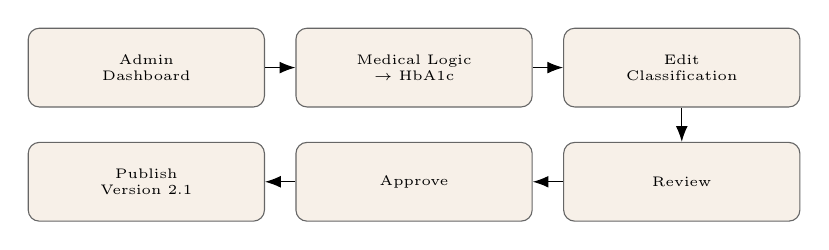
\begin{tikzpicture}[>=Latex]
\node[draw=black!60,rounded corners,fill=brown!12,minimum width=3.0cm,minimum height=1.0cm,align=center,font=\tiny,text width=2.75cm,inner sep=2pt] (s0) at (0.0,0.0) {Admin\\Dashboard};
\node[draw=black!60,rounded corners,fill=brown!12,minimum width=3.0cm,minimum height=1.0cm,align=center,font=\tiny,text width=2.75cm,inner sep=2pt] (s1) at (3.4,0.0) {Medical Logic\\$\to$ HbA1c};
\node[draw=black!60,rounded corners,fill=brown!12,minimum width=3.0cm,minimum height=1.0cm,align=center,font=\tiny,text width=2.75cm,inner sep=2pt] (s2) at (6.8,0.0) {Edit\\Classification};
\node[draw=black!60,rounded corners,fill=brown!12,minimum width=3.0cm,minimum height=1.0cm,align=center,font=\tiny,text width=2.75cm,inner sep=2pt] (s3) at (6.8,-1.45) {Review};
\node[draw=black!60,rounded corners,fill=brown!12,minimum width=3.0cm,minimum height=1.0cm,align=center,font=\tiny,text width=2.75cm,inner sep=2pt] (s4) at (3.4,-1.45) {Approve};
\node[draw=black!60,rounded corners,fill=brown!12,minimum width=3.0cm,minimum height=1.0cm,align=center,font=\tiny,text width=2.75cm,inner sep=2pt] (s5) at (0.0,-1.45) {Publish\\Version 2.1};
\draw[-{Latex[length=2mm]}] (s0.east)--(s1.west);
\draw[-{Latex[length=2mm]}] (s1.east)--(s2.west);
\draw[-{Latex[length=2mm]}] (s2.south)--(s3.north);
\draw[-{Latex[length=2mm]}] (s3.west)--(s4.east);
\draw[-{Latex[length=2mm]}] (s4.west)--(s5.east);
\end{tikzpicture}
\end{adjustbox}
\end{center}
\end{frame}

\begin{frame}[t]{Module 23: Version Control Module}
\textcolor{black!55}{\scriptsize Cluster 6 -- \textcolor{brown}{\textbf{Platform Governance}} (M22--M26) \\ Every report carries its own version stamp}\\[2pt]
\begin{itemize}
\scriptsize
\item Critical for medical software: every report records the medical rule, reference-range, risk-calculator, recommendation and report-engine versions it used
\item Lets the team determine exactly why an old report produced its conclusion after a guideline changes
\end{itemize}
\vspace{4pt}
\begin{center}
\begin{adjustbox}{max width=0.96\linewidth,max height=0.62\textheight}
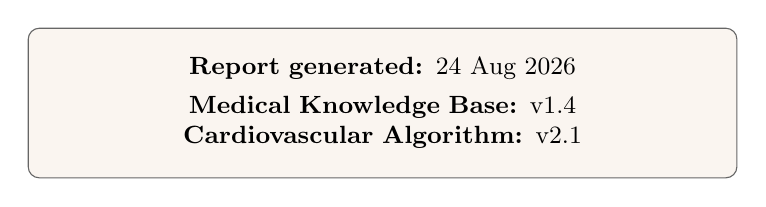
\begin{tikzpicture}[>=Latex]
\node[draw=black!60,rounded corners,fill=brown!8,minimum width=9.0cm,minimum height=1.9cm,align=center,font=\small,text width=8.75cm,inner sep=2pt] (vc1) at (0,0) {\textbf{Report generated:} 24 Aug 2026\\[3pt]\textbf{Medical Knowledge Base:} v1.4\\\textbf{Cardiovascular Algorithm:} v2.1};
\end{tikzpicture}
\end{adjustbox}
\end{center}
\end{frame}

\begin{frame}[t]{Module 24: Audit \& Clinical Decision Log}
\textcolor{black!55}{\scriptsize Cluster 6 -- \textcolor{brown}{\textbf{Platform Governance}} (M22--M26) \\ A full decision trace, retained per conclusion}\\[2pt]
\begin{itemize}
\scriptsize
\item Every important conclusion retains its reasoning inputs
\item Valuable for debugging, medical review, quality assurance, dispute investigation, and algorithm improvement
\end{itemize}
\vspace{4pt}
\begin{center}
\begin{adjustbox}{max width=0.96\linewidth,max height=0.62\textheight}
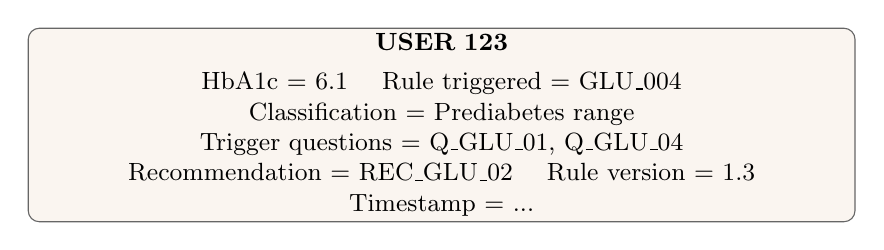
\begin{tikzpicture}[>=Latex]
\node[draw=black!60,rounded corners,fill=brown!8,minimum width=10.5cm,minimum height=2.3cm,align=center,font=\small,text width=10.25cm,inner sep=2pt] (al1) at (0,0) {\textbf{USER 123}\\[3pt]HbA1c = 6.1 \quad Rule triggered = GLU\_004\\Classification = Prediabetes range\\Trigger questions = Q\_GLU\_01, Q\_GLU\_04\\Recommendation = REC\_GLU\_02 \quad Rule version = 1.3\\Timestamp = ...};
\end{tikzpicture}
\end{adjustbox}
\end{center}
\end{frame}

\begin{frame}[t]{Module 25: Security, Privacy \& Permission Module}
\textcolor{black!55}{\scriptsize Cluster 6 -- \textcolor{brown}{\textbf{Platform Governance}} (M22--M26) \\ Nine components under one platform-wide layer}\\[2pt]
\begin{itemize}
\scriptsize
\item A platform-wide backend layer: authentication, encryption, role-based access, consent management, access logs, deletion, export, backup, recovery
\item Medical administrators, programmers and customer support each need different permission levels
\end{itemize}
\vspace{4pt}
\begin{center}
\begin{adjustbox}{max width=0.96\linewidth,max height=0.62\textheight}
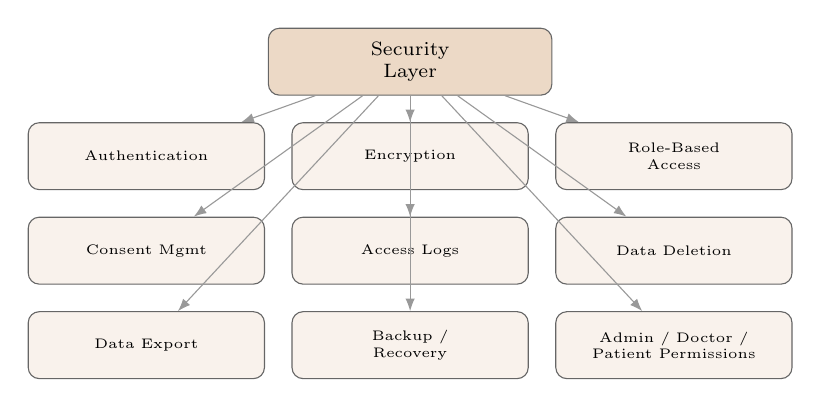
\begin{tikzpicture}[>=Latex]
\node[draw=black!60,rounded corners,fill=brown!10,minimum width=3.0cm,minimum height=0.85cm,align=center,font=\tiny,text width=2.75cm,inner sep=2pt] (g0) at (0.0,0.0) {Authentication};
\node[draw=black!60,rounded corners,fill=brown!10,minimum width=3.0cm,minimum height=0.85cm,align=center,font=\tiny,text width=2.75cm,inner sep=2pt] (g1) at (3.35,0.0) {Encryption};
\node[draw=black!60,rounded corners,fill=brown!10,minimum width=3.0cm,minimum height=0.85cm,align=center,font=\tiny,text width=2.75cm,inner sep=2pt] (g2) at (6.7,0.0) {Role-Based\\Access};
\node[draw=black!60,rounded corners,fill=brown!10,minimum width=3.0cm,minimum height=0.85cm,align=center,font=\tiny,text width=2.75cm,inner sep=2pt] (g3) at (0.0,-1.2) {Consent Mgmt};
\node[draw=black!60,rounded corners,fill=brown!10,minimum width=3.0cm,minimum height=0.85cm,align=center,font=\tiny,text width=2.75cm,inner sep=2pt] (g4) at (3.35,-1.2) {Access Logs};
\node[draw=black!60,rounded corners,fill=brown!10,minimum width=3.0cm,minimum height=0.85cm,align=center,font=\tiny,text width=2.75cm,inner sep=2pt] (g5) at (6.7,-1.2) {Data Deletion};
\node[draw=black!60,rounded corners,fill=brown!10,minimum width=3.0cm,minimum height=0.85cm,align=center,font=\tiny,text width=2.75cm,inner sep=2pt] (g6) at (0.0,-2.4) {Data Export};
\node[draw=black!60,rounded corners,fill=brown!10,minimum width=3.0cm,minimum height=0.85cm,align=center,font=\tiny,text width=2.75cm,inner sep=2pt] (g7) at (3.35,-2.4) {Backup /\\Recovery};
\node[draw=black!60,rounded corners,fill=brown!10,minimum width=3.0cm,minimum height=0.85cm,align=center,font=\tiny,text width=2.75cm,inner sep=2pt] (g8) at (6.7,-2.4) {Admin / Doctor /\\Patient Permissions};
\node[draw=black!60,rounded corners,fill=brown!30,minimum width=3.6cm,minimum height=0.85cm,align=center,font=\scriptsize,text width=3.35cm,inner sep=2pt] (gc) at (3.35,1.2) {Security\\Layer};
\draw[-{Latex[length=1.6mm]},black!40] (gc)--(g0);
\draw[-{Latex[length=1.6mm]},black!40] (gc)--(g1);
\draw[-{Latex[length=1.6mm]},black!40] (gc)--(g2);
\draw[-{Latex[length=1.6mm]},black!40] (gc)--(g3);
\draw[-{Latex[length=1.6mm]},black!40] (gc)--(g4);
\draw[-{Latex[length=1.6mm]},black!40] (gc)--(g5);
\draw[-{Latex[length=1.6mm]},black!40] (gc)--(g6);
\draw[-{Latex[length=1.6mm]},black!40] (gc)--(g7);
\draw[-{Latex[length=1.6mm]},black!40] (gc)--(g8);
\end{tikzpicture}
\end{adjustbox}
\end{center}
\end{frame}

\begin{frame}[t]{Module 26: Analytics \& System Improvement Module}
\textcolor{black!55}{\scriptsize Cluster 6 -- \textcolor{brown}{\textbf{Platform Governance}} (M22--M26) \\ System-level insight, never clinical decision-making}\\[2pt]
\begin{itemize}
\scriptsize
\item Anonymised, system-level analytics: common abnormalities, risk combinations, question completion rate, upload success rate, referral rates, retention, repeat-testing behaviour
\item \textbf{Kept separate from clinical decision-making}
\end{itemize}
\vspace{4pt}
\begin{center}
\begin{adjustbox}{max width=0.96\linewidth,max height=0.62\textheight}
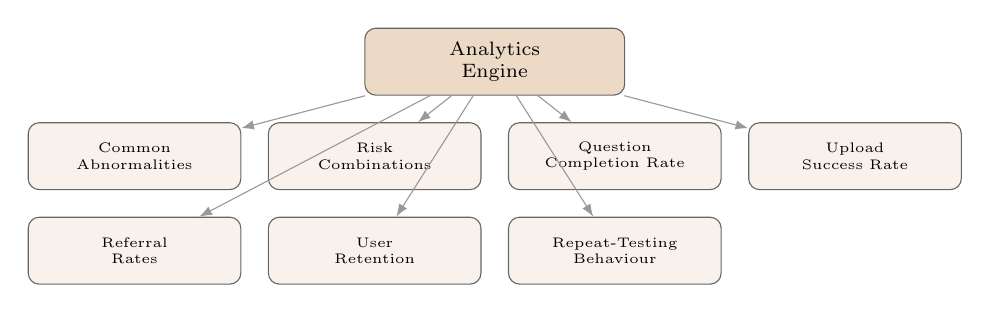
\begin{tikzpicture}[>=Latex]
\node[draw=black!60,rounded corners,fill=brown!10,minimum width=2.7cm,minimum height=0.85cm,align=center,font=\tiny,text width=2.45cm,inner sep=2pt] (g0) at (0.0,0.0) {Common\\Abnormalities};
\node[draw=black!60,rounded corners,fill=brown!10,minimum width=2.7cm,minimum height=0.85cm,align=center,font=\tiny,text width=2.45cm,inner sep=2pt] (g1) at (3.0500000000000003,0.0) {Risk\\Combinations};
\node[draw=black!60,rounded corners,fill=brown!10,minimum width=2.7cm,minimum height=0.85cm,align=center,font=\tiny,text width=2.45cm,inner sep=2pt] (g2) at (6.1000000000000005,0.0) {Question\\Completion Rate};
\node[draw=black!60,rounded corners,fill=brown!10,minimum width=2.7cm,minimum height=0.85cm,align=center,font=\tiny,text width=2.45cm,inner sep=2pt] (g3) at (9.15,0.0) {Upload\\Success Rate};
\node[draw=black!60,rounded corners,fill=brown!10,minimum width=2.7cm,minimum height=0.85cm,align=center,font=\tiny,text width=2.45cm,inner sep=2pt] (g4) at (0.0,-1.2) {Referral\\Rates};
\node[draw=black!60,rounded corners,fill=brown!10,minimum width=2.7cm,minimum height=0.85cm,align=center,font=\tiny,text width=2.45cm,inner sep=2pt] (g5) at (3.0500000000000003,-1.2) {User\\Retention};
\node[draw=black!60,rounded corners,fill=brown!10,minimum width=2.7cm,minimum height=0.85cm,align=center,font=\tiny,text width=2.45cm,inner sep=2pt] (g6) at (6.1000000000000005,-1.2) {Repeat-Testing\\Behaviour};
\node[draw=black!60,rounded corners,fill=brown!30,minimum width=3.3000000000000003cm,minimum height=0.85cm,align=center,font=\scriptsize,text width=3.0500000000000003cm,inner sep=2pt] (gc) at (4.575,1.2) {Analytics\\Engine};
\draw[-{Latex[length=1.6mm]},black!40] (gc)--(g0);
\draw[-{Latex[length=1.6mm]},black!40] (gc)--(g1);
\draw[-{Latex[length=1.6mm]},black!40] (gc)--(g2);
\draw[-{Latex[length=1.6mm]},black!40] (gc)--(g3);
\draw[-{Latex[length=1.6mm]},black!40] (gc)--(g4);
\draw[-{Latex[length=1.6mm]},black!40] (gc)--(g5);
\draw[-{Latex[length=1.6mm]},black!40] (gc)--(g6);
\end{tikzpicture}
\end{adjustbox}
\end{center}
\end{frame}

\section{Architecture Principles}

\begin{frame}[t]{The Four-Layer Model}
\textcolor{black!55}{\scriptsize Think of the platform as four layers, not one application}\\[2pt]
\begin{center}
\begin{adjustbox}{max width=0.96\linewidth,max height=0.62\textheight}
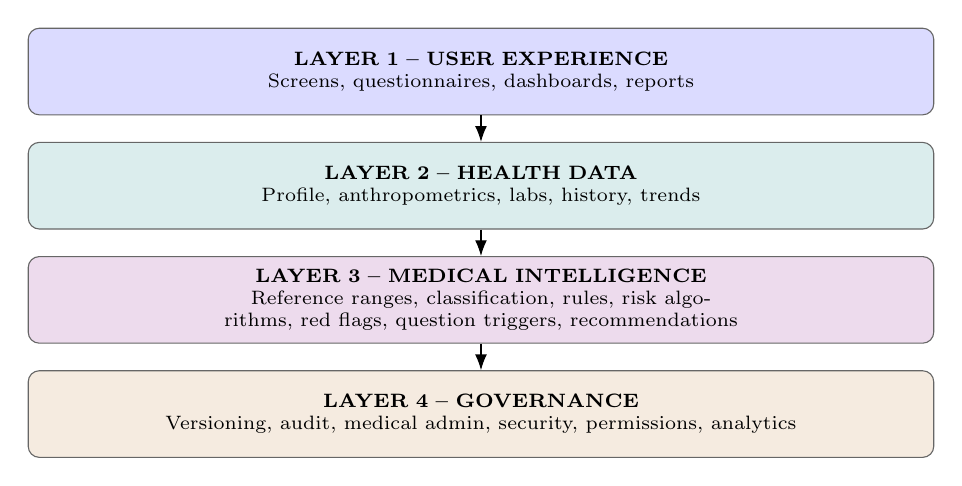
\begin{tikzpicture}[>=Latex]
\node[draw=black!60,rounded corners,fill=blue!14,minimum width=11.5cm,minimum height=1.1cm,align=center,font=\scriptsize,text width=11.25cm,inner sep=2pt] (lv0) at (0,0) {\textbf{LAYER 1 -- USER EXPERIENCE}\\Screens, questionnaires, dashboards, reports};
\node[draw=black!60,rounded corners,fill=teal!14,minimum width=11.5cm,minimum height=1.1cm,align=center,font=\scriptsize,text width=11.25cm,inner sep=2pt] (lv1) at (0,-1.4500000000000002) {\textbf{LAYER 2 -- HEALTH DATA}\\Profile, anthropometrics, labs, history, trends};
\node[draw=black!60,rounded corners,fill=violet!14,minimum width=11.5cm,minimum height=1.1cm,align=center,font=\scriptsize,text width=11.25cm,inner sep=2pt] (lv2) at (0,-2.9000000000000004) {\textbf{LAYER 3 -- MEDICAL INTELLIGENCE}\\Reference ranges, classification, rules, risk algorithms, red flags, question triggers, recommendations};
\node[draw=black!60,rounded corners,fill=brown!16,minimum width=11.5cm,minimum height=1.1cm,align=center,font=\scriptsize,text width=11.25cm,inner sep=2pt] (lv3) at (0,-4.3500000000000005) {\textbf{LAYER 4 -- GOVERNANCE}\\Versioning, audit, medical admin, security, permissions, analytics};
\draw[-{Latex[length=2mm]}] (lv0.south)--(lv1.north);
\draw[-{Latex[length=2mm]}] (lv1.south)--(lv2.north);
\draw[-{Latex[length=2mm]}] (lv2.south)--(lv3.north);
\end{tikzpicture}
\end{adjustbox}
\end{center}
\end{frame}

\begin{frame}[t]{Never Hard-Code Medical Knowledge}
\textcolor{black!55}{\scriptsize The single most important rule for developers}\\[2pt]
\begin{center}
\begin{adjustbox}{max width=0.96\linewidth,max height=0.62\textheight}
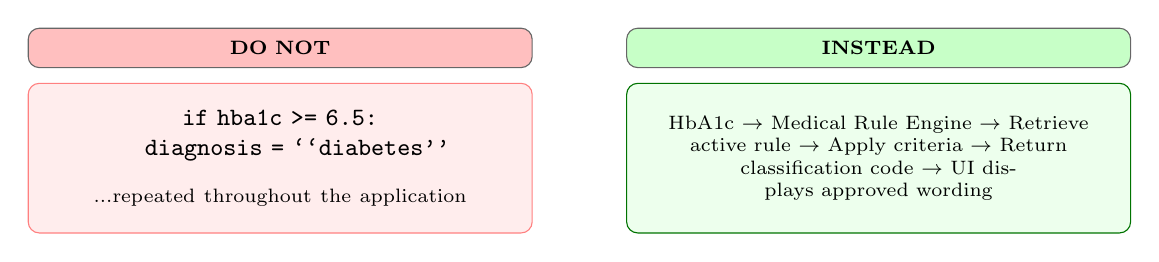
\begin{tikzpicture}[>=Latex]
\node[draw=black!60,rounded corners,fill=red!25,minimum width=6.4cm,minimum height=0.5cm,align=center,font=\scriptsize,text width=6.15cm,inner sep=2pt] (hc_bad_t) at (0,1.5) {\textbf{DO NOT}};
\node[draw=red!50,rounded corners,fill=red!7,minimum width=6.4cm,minimum height=1.9cm,align=center,font=\small,text width=6.15cm,inner sep=2pt] (hc_bad) at (0,0.1) {\texttt{if hba1c >= 6.5:}\\\texttt{\ \ \ \ diagnosis = ``diabetes''}\\[6pt]\scriptsize ...repeated throughout the application};
\node[draw=black!60,rounded corners,fill=green!22,minimum width=6.4cm,minimum height=0.5cm,align=center,font=\scriptsize,text width=6.15cm,inner sep=2pt] (hc_good_t) at (7.6,1.5) {\textbf{INSTEAD}};
\node[draw=green!45!black,rounded corners,fill=green!7,minimum width=6.4cm,minimum height=1.9cm,align=center,font=\scriptsize,text width=6.15cm,inner sep=2pt] (hc_good) at (7.6,0.1) {HbA1c $\to$ Medical Rule Engine $\to$ Retrieve\\active rule $\to$ Apply criteria $\to$ Return\\classification code $\to$ UI displays approved wording};
\end{tikzpicture}
\end{adjustbox}
\end{center}
\begin{center}
\begin{adjustbox}{max width=0.96\linewidth,max height=0.18\textheight}

\begin{tikzpicture}[>=Latex]
\node[draw=blue!30,rounded corners,fill=blue!5,minimum width=14.0cm,minimum height=0.85cm,align=center,font=\scriptsize,text width=13.75cm,inner sep=2pt] (hc_note) at (3.8,-2.2) {\scriptsize Scalable: update WHO/MOH guideline standards, introduce new risk calculators, add new blood tests, or change recommendation wording -- without rebuilding the platform.};
\end{tikzpicture}
\end{adjustbox}
\end{center}
\end{frame}

\section{Team Division}

\begin{frame}[t]{Team Division (Four-Person Team)}
\textcolor{black!55}{\scriptsize This architecture creates a clean ownership split}\\[2pt]
\begin{center}
\begin{adjustbox}{max width=0.96\linewidth,max height=0.62\textheight}
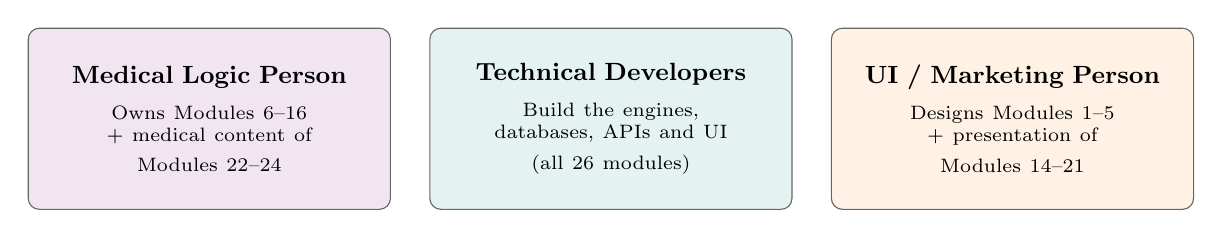
\begin{tikzpicture}[>=Latex]
\node[draw=black!60,rounded corners,fill=violet!10,minimum width=4.6cm,minimum height=2.3cm,align=center,font=\small,text width=4.35cm,inner sep=2pt] (tm1) at (0,0) {\textbf{Medical Logic Person}\\[5pt]\scriptsize Owns Modules 6--16\\+ medical content of\\Modules 22--24};
\node[draw=black!60,rounded corners,fill=teal!10,minimum width=4.6cm,minimum height=2.3cm,align=center,font=\small,text width=4.35cm,inner sep=2pt] (tm2) at (5.1,0) {\textbf{Technical Developers}\\[5pt]\scriptsize Build the engines,\\databases, APIs and UI\\(all 26 modules)};
\node[draw=black!60,rounded corners,fill=orange!10,minimum width=4.6cm,minimum height=2.3cm,align=center,font=\small,text width=4.35cm,inner sep=2pt] (tm3) at (10.2,0) {\textbf{UI / Marketing Person}\\[5pt]\scriptsize Designs Modules 1--5\\+ presentation of\\Modules 14--21};
\end{tikzpicture}
\end{adjustbox}
\end{center}
\end{frame}


\begin{frame}
\centering
\Huge Thank You
\vspace{10pt}

\normalsize \textit{MyHealthReport --- Technical Module Architecture}
\end{frame}

\end{document}
